\documentclass{article}

\usepackage{arxiv}

\usepackage[utf8]{inputenc} % allow utf-8 input
\usepackage[T1]{fontenc}    % use 8-bit T1 fonts
\usepackage{lmodern}        % https://github.com/rstudio/rticles/issues/343
\usepackage{hyperref}       % hyperlinks
\usepackage{url}            % simple URL typesetting
\usepackage{booktabs}       % professional-quality tables
\usepackage{amsfonts}       % blackboard math symbols
\usepackage{nicefrac}       % compact symbols for 1/2, etc.
\usepackage{microtype}      % microtypography
\usepackage{graphicx}

\title{Missing links and the topological robustness of food webs}

\author{
    Anubhav Gupta
    \thanks{Corresponding author}
   \\
    Department of Evolutionary Biology and Environmental Studies \\
    University of Zurich \\
  8057 Zurich, Switzerland \\
  \texttt{\href{mailto:anubhav.gupta@ieu.uzh.ch}{\nolinkurl{anubhav.gupta@ieu.uzh.ch}}} \\
   \And
    Owen L. Petchey
   \\
    Department of Evolutionary Biology and Environmental Studies \\
    University of Zurich \\
  8057 Zurich, Switzerland \\
  \texttt{\href{mailto:owen.petchey@ieu.uzh.ch}{\nolinkurl{owen.petchey@ieu.uzh.ch}}} \\
  }


% tightlist command for lists without linebreak
\providecommand{\tightlist}{%
  \setlength{\itemsep}{0pt}\setlength{\parskip}{0pt}}


% Pandoc citation processing
\newlength{\cslhangindent}
\setlength{\cslhangindent}{1.5em}
\newlength{\csllabelwidth}
\setlength{\csllabelwidth}{3em}
\newlength{\cslentryspacingunit} % times entry-spacing
\setlength{\cslentryspacingunit}{\parskip}
% for Pandoc 2.8 to 2.10.1
\newenvironment{cslreferences}%
  {}%
  {\par}
% For Pandoc 2.11+
\newenvironment{CSLReferences}[2] % #1 hanging-ident, #2 entry spacing
 {% don't indent paragraphs
  \setlength{\parindent}{0pt}
  % turn on hanging indent if param 1 is 1
  \ifodd #1
  \let\oldpar\par
  \def\par{\hangindent=\cslhangindent\oldpar}
  \fi
  % set entry spacing
  \setlength{\parskip}{#2\cslentryspacingunit}
 }%
 {}
\usepackage{calc}
\newcommand{\CSLBlock}[1]{#1\hfill\break}
\newcommand{\CSLLeftMargin}[1]{\parbox[t]{\csllabelwidth}{#1}}
\newcommand{\CSLRightInline}[1]{\parbox[t]{\linewidth - \csllabelwidth}{#1}\break}
\newcommand{\CSLIndent}[1]{\hspace{\cslhangindent}#1}

\usepackage{lineno}
\linenumbers
\usepackage {amsmath}
\setlength\parindent{24pt}
\usepackage{setspace}\doublespacing
\usepackage{booktabs}
\usepackage{longtable}
\usepackage{array}
\usepackage{multirow}
\usepackage{wrapfig}
\usepackage{float}
\usepackage{colortbl}
\usepackage{pdflscape}
\usepackage{tabu}
\usepackage{threeparttable}
\usepackage{threeparttablex}
\usepackage[normalem]{ulem}
\usepackage{makecell}
\usepackage{xcolor}
\begin{document}
\maketitle


\begin{abstract}
\begin{enumerate}
\def\labelenumi{\arabic{enumi})}
\tightlist
\item
  Undersampling can lead to missing trophic interactions in recorded
  food webs, with potential consequences for the perceived functioning
  and stability of the food webs. Undersampling can be compensated for
  by using food web models such as the allometric diet breadth model
  (ADBM) to predict missing links. Simultaneously, models might predict
  links which cannot occur, i.e., false positives.
\item
  Previous research shows that (i) food web robustness (the inverse of
  the number of secondary extinctions occurring due to primary
  extinctions) increases with connectance (the number of realised
  trophic links divided by the number of possible links), and (ii) that
  model predicted food webs usually have greater connectance than
  observed ones. Thus, we expect that predicted food webs are more
  robust than observed ones. However, this expectation has never, to our
  knowledge, been tested, nor has the effect size, i.e.~the difference
  in robustness of predicted and observed food web with respect to the
  difference in their connectance, been quantified.
\item
  We fill this research gap by comparing the robustness of observed food
  webs to the robustness of food webs predicted by a model (the ADBM)
  that can account for missing links but does not predict all links
  correctly. We did this for 12 different food webs from a wide variety
  of ecosystems. We used three extinction scenarios: random, most
  connected, and least connected.
\item
  We found, as expected, that the predicted food webs were more robust
  than the observed food webs, which can be attributed to the higher
  connectance of the predicted food webs. On average, for every one unit
  of increase in connectance, we found that the food webs robustness
  increased by 0.52 units for the most connected species extinction
  scenario and by 0.04 units for the random species extinction
  scenarios. On the other hand, we saw no effect, on average, of
  increased connectance for the least connected species extinction
  scenario for all except two of the 12 food webs.
\item
  These results show that undersampling can lead to large underestimates
  of food web robustness that can be compensated for by filling in
  missing links with food web models. Nevertheless, increased
  connectance may contribute to lower dynamical stability, so it would
  be interesting to compare the dynamical stability of observed and
  predicted food webs and the topological stability that we have focused
  on.
\end{enumerate}
\end{abstract}

\keywords{
    connectance
   \and
    ABC
   \and
    ADBM
   \and
    food web
   \and
    extinction
   \and
    uncertainty
  }

\hypertarget{introduction}{%
\section{Introduction}\label{introduction}}

Anthropogenic changes such as climate change and habitat destruction are
a threat to biodiversity and can lead to food web collapse (Ullah et
al., 2018). This food web collapse is due to the cascades of secondary
extinctions in a food web because of the primary loss of species due to
environmental change (Pimm et al., 2006; C. D. Thomas et al., 2004; J.
A. Thomas et al., 2004). An example of a secondary extinction is when a
consumer goes extinct because its sole resource species goes extinct.
Therefore, research focused on cascading secondary extinctions, also
known as `community viability analysis', has been performed extensively
in the past few decades to quantify how robust food webs are to species
extinction (Berg et al., 2011; Dunne et al., 2002a; Dunne \& Williams,
2009; Ebenman et al., 2004; Ebenman \& Jonsson, 2005). This research
revealed that the rate of collapse of a food web depends on its
structure and complexity (Dunne et al., 2002a; Dunne \& Williams, 2009).

Simulation of primary species loss has been conducted in observed food
webs and model food webs from terrestrial and aquatic ecosystems, where
robustness was measured in terms of secondary extinctions (Dunne et al.,
2002a; Dunne \& Williams, 2009). Primary species loss is considered to
be extinction of a species due to causes external to the food web,
e.g.~overharvesting (Koning \& McIntyre, 2021), introduction of invasive
species (David et al., 2017). A secondary extinction is an extinction
caused by a previous extinction (either primary or secondary). Numerous
studies have used topological criterion for assigning a secondary
extinction to a species, i.e., if extinction is of the last resource
species of a consumer species, then the consumer species suffers
secondary extinction (Dunne et al., 2002a; Dunne \& Williams, 2009;
Sol'e \& Montoya, 2001).

When there are few primary extinctions, and these cause many secondary
extinctions, a food web is said to be fragile or not robust. In
contrast, a food web is said to be robust when there are only a few
secondary extinctions. Several studies have shown that the robustness of
the food webs increases with food web connectance (Dunne et al., 2002b;
Dunne \& Williams, 2009). Additionally, these studies have demonstrated
that the removal (primary extinction) of the most connected species
causes considerably more secondary extinctions than the random removals
of species (Dunne et al., 2002b; Sol'e \& Montoya, 2001). Simulation
studies like these, which investigate the impact of primary extinctions
in a food web to quantify robustness based on its topological structure,
provide an alternate solution to canonical experiments in natural
ecosystems, which are not possible or very difficult to conduct (Dunne
\& Williams, 2009).

Along with quantifying food web robustness based on its topological
structure, studies such as Williams (2008), Brose et al. (2006), and
Martinez et al. (2006) have quantified robustness based on the abundance
dynamics of a food web. However, the topological approach of quantifying
a food web's robustness only requires the food web structure, whereas
the dynamical approach requires the food web structure and the temporal
dynamics of the abundance of species in that food web. For example,
Williams (2008) combined network structure models with bioenergetic
dynamics models to study the role of food web topology and nonlinear
dynamics on species coexistence in complex ecological networks.

A key assumption of the observed food webs is that they are very well
sampled, i.e.~all the links that in reality can occur are represented.
However, it is known that not all food webs are very well sampled and do
not represent all of the feeding links that can occur (Caron et al.,
2022; Jordano, 2016; Patonai \& Jord'an, 2017). Some rare trophic links
require more sampling effort than others, whereas some trophic links
remain unobserved because of biological constraints such as
spatio-temporal uncoupling, size or reward mismatching, foraging
constraints and physiological-biochemical constraints, which are
irrespective of sufficient sampling effort (Jordano, 2016). Previous
studies such as Caron et al. (2022) and Gupta et al. (2022) have shown
that the predicted food webs from these models usually have greater
connectance than the observed ones. One solution to compensate for
undersampling is using a food web model such as the Allometric Diet
Breadth Model (ADBM) (Petchey et al., 2008) to predict the missing links
and then measure the robustness of the predicted food web. The ADBM is a
mechanistic model constructed using foraging rules based on the body
sizes of prey and predator, where trophic interactions satisfying those
rules would be predicted by the model, which are perhaps not observed
because those interactions are rare. However, this solution is not
infallible, as it is likely that the food web model might still miss
some links and also may predict some links that could not, in fact
occur.

In our study, we investigate the topological robustness of the ADBM
predicted food webs and compare it to that of the observed food webs. We
expect the ADBM predicted food webs to be more robust than the observed
food webs, and for the greater robustness to be related to the amount by
which the ADBM predicts greater connectance compared to that of the
observed food webs. We do this by simulating primary species loss in 12
food webs predicted by the ADBM to quantify the secondary loss of
extinctions and compare the robustness of food webs predicted by the
ADBM to the robustness of the observed food webs. We use three different
approaches of primary species removal: (i) most connected species, (ii)
random species and (iii) least connected species to understand if the
outcome varies among these approaches.

\hypertarget{materials-and-methods}{%
\section{Materials and methods}\label{materials-and-methods}}

In the upcoming sections, we present a detailed account of the
implementation of the simulation of primary extinctions for three
different extinction scenarios on 12 food webs predicted by the ADBM
from a wide variety of ecosystems and compute the resultant secondary
extinctions. We then describe a robustness metric of those predicted
food webs and how we compare them to the properties of the food webs.

\hypertarget{allometric-diet-breadth-model-adbm}{%
\subsection{Allometric Diet Breadth Model
(ADBM)}\label{allometric-diet-breadth-model-adbm}}

The allometric diet breadth model (ADBM) is based on optimal foraging
theory, specifically the contingency model (MacArthur \& Pianka, 1966).
We chose this model because it is known to predict greater connectance
in the predicted food webs compared to the observed food webs (Gupta et
al., 2022). The ADBM predicts the set of prey species a consumer should
feed upon to maximise its rate of energy intake (Petchey et al., 2008).
The foraging variables used in the model are the energy content of prey,
handling times of the predator on prey, space clearance rate, i.e.~how
fast a predator searches space, and prey densities. Each of these
variables is derived from the allometric scaling relationship using the
body sizes of species. More details on the foraging rules defined in the
ADBM and ADBM's predictive power across different food webs can be found
in open access Petchey et al. (2008).

\hypertarget{food-web-data}{%
\subsection{Food web data}\label{food-web-data}}

The observed food webs that we fit the ADBM to belong to marine,
freshwater and terrestrial ecosystems (Table \ref{fig:tab_1}). We
considered these food webs because they belong to diverse ecosystems and
follow FAIR (Findable Accessible Interoperable Reusable) principles
(Wilkinson et al., 2016). These food webs contain primary producers,
herbivores, carnivores, parasites, and parasitoids and various feeding
interactions, including predation, herbivory, bacterivory, parasitism
and pathogenic. The observed connectance of these food webs varies from
0.03 to 0.24 (Links/Species\(^2\)), and the number of species varies
from 29 to 239. The goodness of fit of the ADBM's predictions depends on
the interaction types in the food webs. For example, those with
size-structured interactions, such as herbivory in aquatic ecosystems,
are better predicted compared to less size-structured ones, such as
parasitoids and terrestrial herbivory ones (Petchey et al., 2008).

\newgeometry{margin=1cm}
\begin{landscape}\begin{table}

\caption{\label{tab:unnamed-chunk-1}\label{fig:tab_1}Information about the food webs predicted using the ADBM.}
\centering
\resizebox{\linewidth}{!}{
\fontsize{7}{9}\selectfont
\begin{tabular}[t]{>{\raggedright\arraybackslash}p{4cm}|>{\raggedright\arraybackslash}p{3cm}|l|>{\raggedright\arraybackslash}p{2cm}|>{\raggedright\arraybackslash}p{2cm}|>{\raggedright\arraybackslash}p{3cm}}
\hline
Common food web name (Original Publication) & Predation matrix source & General ecosystem & Number of species & Observed connectance (Links/Species$^2$) & 95\% prediction interval of predicted connectance  of the ADBM  (Gupta et al. 2022)\\
\hline
Benguela Pelagic (Yodzis 1998) & Brose et al. (2005) & Marine & 30 & 0.21 & 0.26 - 0.59\\
\hline
Broadstone Stream (taxonomic aggregation) (Woodward and Hildrew 2001; Woodward
et al. 2005) & Brose et al. (2005) & Freshwater & 29 & 0.19 & 0.18 - 0.72\\
\hline
Broom (Memmott et al. 2000) & Brose et al. (2005) & Terrestrial & 60 & 0.03 & 0.12 - 0.89\\
\hline
Capinteria (Lafferty et al. 2006) & Hechinger et al. (2011) & Marine (Salt Marsh) & 88 & 0.08 & 0.11 - 0.80\\
\hline
Caricaie Lakes (Cattin et al. 2004) & Brose et al. (2005) & Freshwater & 158 & 0.05 & 0.11 - 0.81\\
\hline
Grasslands (Dawah et al. 1995) & Brose et al. (2005) & Terrestrial & 65 & 0.03 & 0.03 - 0.44\\
\hline
Mill Stream (Ledger, Edwards, Woodward unpublished) & Brose et al. (2005) & Freshwater & 80 & 0.06 & 0.08 - 0.60\\
\hline
Skipwith Pond (Warren 1989) & Brose et al. (2005) & Freshwater & 71 & 0.07 & 0.17 - 0.90\\
\hline
Small Reef (Opitz 1996 Table 8.6.2) & Alyssa R. Cirtwill and Anna Eklöf (2018) & Marine (Reef) & 239 & 0.06 & 0.07 - 0.66\\
\hline
Tuesday Lake (Jonsson et al. 2005) & Brose et al. (2005) & Freshwater & 73 & 0.08 & 0.09 - 0.57\\
\hline
Ythan (Emmerson and Raffaelli 2004) & Alyssa R. Cirtwill and Anna Eklöf (2018) & Marine (Estuarine) & 85 & 0.04 & 0.13 - 0.84\\
\hline
Broadstone Stream (size aggregation) (Woodward
et al. 2010) & Guy Woodward (2021) & Freshwater & 29 & 0.24 & 0.25 - 0.47\\
\hline
\end{tabular}}
\end{table}
\end{landscape}
\restoregeometry

\hypertarget{model-parameterisation-using-approximate-bayesian-computation}{%
\subsection{Model parameterisation using approximate Bayesian
computation}\label{model-parameterisation-using-approximate-bayesian-computation}}

The ADBM was parameterised using approximate Bayesian computation (ABC),
where a set of parameter values were sampled from a prior distribution.
Then, that set of parameter values was either accepted or rejected based
on how close the predicted food web was to the observed food web using
an accuracy metric -- true skill statistic (TSS). The accepted parameter
values formed a posterior distribution (Fig. 4 and S14-S25 in Gupta et
al. (2022)). Further, prediction intervals of the true skill statistic
and connectance of the predicted food webs were computed (Fig. 5 (a, b)
in Gupta et al. (2022)). In our study, we considered model predicted
food webs where the predicted connectance lay within the 95\% prediction
interval of all model predicted food webs. A detailed explanation of the
parameterisation method can be found in Gupta et al. (2022).

\hypertarget{extinction-scenarios-and-robustness}{%
\subsection{Extinction scenarios and
robustness}\label{extinction-scenarios-and-robustness}}

We implemented the primary species removal method from Dunne \& Williams
(2009) by sequentially removing species using one of the three criteria:
removal of (i) the most connected species, (ii) the least connected
species and (iii) randomly chosen species. The most connected and least
connected criteria are based on species' degree (i.e.~the total number
of links to resources and from consumers). We considered these three
criteria because the random extinction scenario takes into account all
the theoretically possible extinction sequences of species that can
occur in a food web, while the extinction of the most connected species
and least connected species takes into account the two opposite extreme
scenarios. These extinction scenarios have been widely used in studying
species extinctions and the collapse of food webs and other networks
(Albert \& Barab'asi, 2002; J. Dunne et al., 2004; Dunne et al., 2002a;
Dunne \& Williams, 2009; Sol'e \& Montoya, 2001).

Given a primary removal of species in a food web, if any remaining
species lost all of their resource species, or any cannibalistic species
lost all of their resource species except the cannibalistic links, they
are removed from the web, and a secondary extinction was recorded.
Secondary extinctions may cause further secondary extinctions, which
were also checked for and recorded. Once no more secondary extinctions
occurred, then another primary extinction was made of the next
appropriate species depending on the extinction scenario. This process
was carried out until all the species were extinct from the food web.

The robustness (R) of a food web was defined as the proportion of
species subjected to primary removals resulting in extinction (primary
and secondary extinctions) of some specified proportion of the species.
In our study, we use \(R_{50}\), the number of primary extinctions
divided by the total number of species, which results in at least 50\%
of total species loss (J. Dunne et al., 2004; Dunne et al., 2002a; Dunne
\& Williams, 2009; Jonsson et al., 2015). Therefore, if primary
extinctions never cause any secondary extinctions, the food web is
maximally robust and (\(R_{50} = 0.50\)). Whereas in a minimally robust
community (\(R_{50} = 1/S\), where \(S\) is the number of species), the
first primary extinction causes a cascade of secondary extinctions of at
least nearly half of the species in the food web (i.e.~at least
\(S/2 - 1\)).

\hypertarget{simulating-species-extinctions}{%
\subsection{Simulating species
extinctions}\label{simulating-species-extinctions}}

First, we simulated primary species loss in food webs predicted by the
ADBM which had the maximum true skill statistics and compared it to
primary species loss in observed food webs. Second, to take into account
the uncertainty in robustness in the ADBM predicted food webs, we
simulated primary species loss and thereby computed robustness for all
the ADBM predicted food webs corresponding to the 95\% prediction
interval of the predicted connectance. Furthermore, in the case of the
random extinction scenario, we simulated 1000 random extinction
sequences in a single ADBM predicted food web.

\hypertarget{analysis}{%
\subsection{Analysis}\label{analysis}}

In the random extinction scenario, we computed robustness \(R_{50}\) for
all 1000 independent random extinction sequences and calculated the
median as a summary statistics to quantify the average robustness of a
single food web to random extinction. To quantify the effect of
undersampling, i.e.~greater connectance of connectance, we compute the
ratio of the difference in normalised robustness between the ADBM
predicted food webs and observed food webs to the difference in their
normalised connectance, where normalisation was performed by dividing
the variables by their maximum possible values (i.e.~0.5 for \(R_{50}\)
and 1 for connectance). However, we did not perform any statistical
significance test because we work with simulated food webs and
therefore, the p-values of these tests are influenced by the number of
model simulations (White et al., 2014).

\hypertarget{results}{%
\section{Results}\label{results}}

We first present the secondary extinction curves of the ADBM predicted
food webs which had the maximum true skill statistics and of the
observed food webs for 12 food webs under three different extinction
scenarios. We then compare the robustness of all the ADBM predicted food
webs within the 95\% prediction interval against that of the observed
food webs to take into account uncertainty in the robustness across food
webs predictions. Finally, we quantify the effect of the difference in
their connectance on the difference in their robustness estimates.

\hypertarget{secondary-extinctions}{%
\subsection{Secondary extinctions}\label{secondary-extinctions}}

In the most connected extinction scenario, the cumulative secondary
extinction curves started to rise steeply in the observed food webs at a
lower number of primary species removal as compared to the ADBM
predicted food webs for nine food webs (Fig. \ref{fig:fig_r1} (a, c, d,
e, f, g, h, j, l)). However, there was a higher number of cumulative
secondary extinctions occurring in the ADBM predicted food webs when
compared to that of the observed food webs at a high number of primary
species removal in five food webs (Fig. \ref{fig:fig_r1} (a, f, g, h,
k)). In the Skipwith Pond food web, there were no secondary extinctions
for any number of primary removal of species (Fig. \ref{fig:fig_r1}
(i)), whereas in the Broadstone Stream (taxonomic aggregation) food web
the same was true only for the observed food web but in the ADBM
predicted food web there was a steep rise in the cumulative secondary
extinctions (Fig. \ref{fig:fig_r1} (b)).

\begin{figure}

{\centering 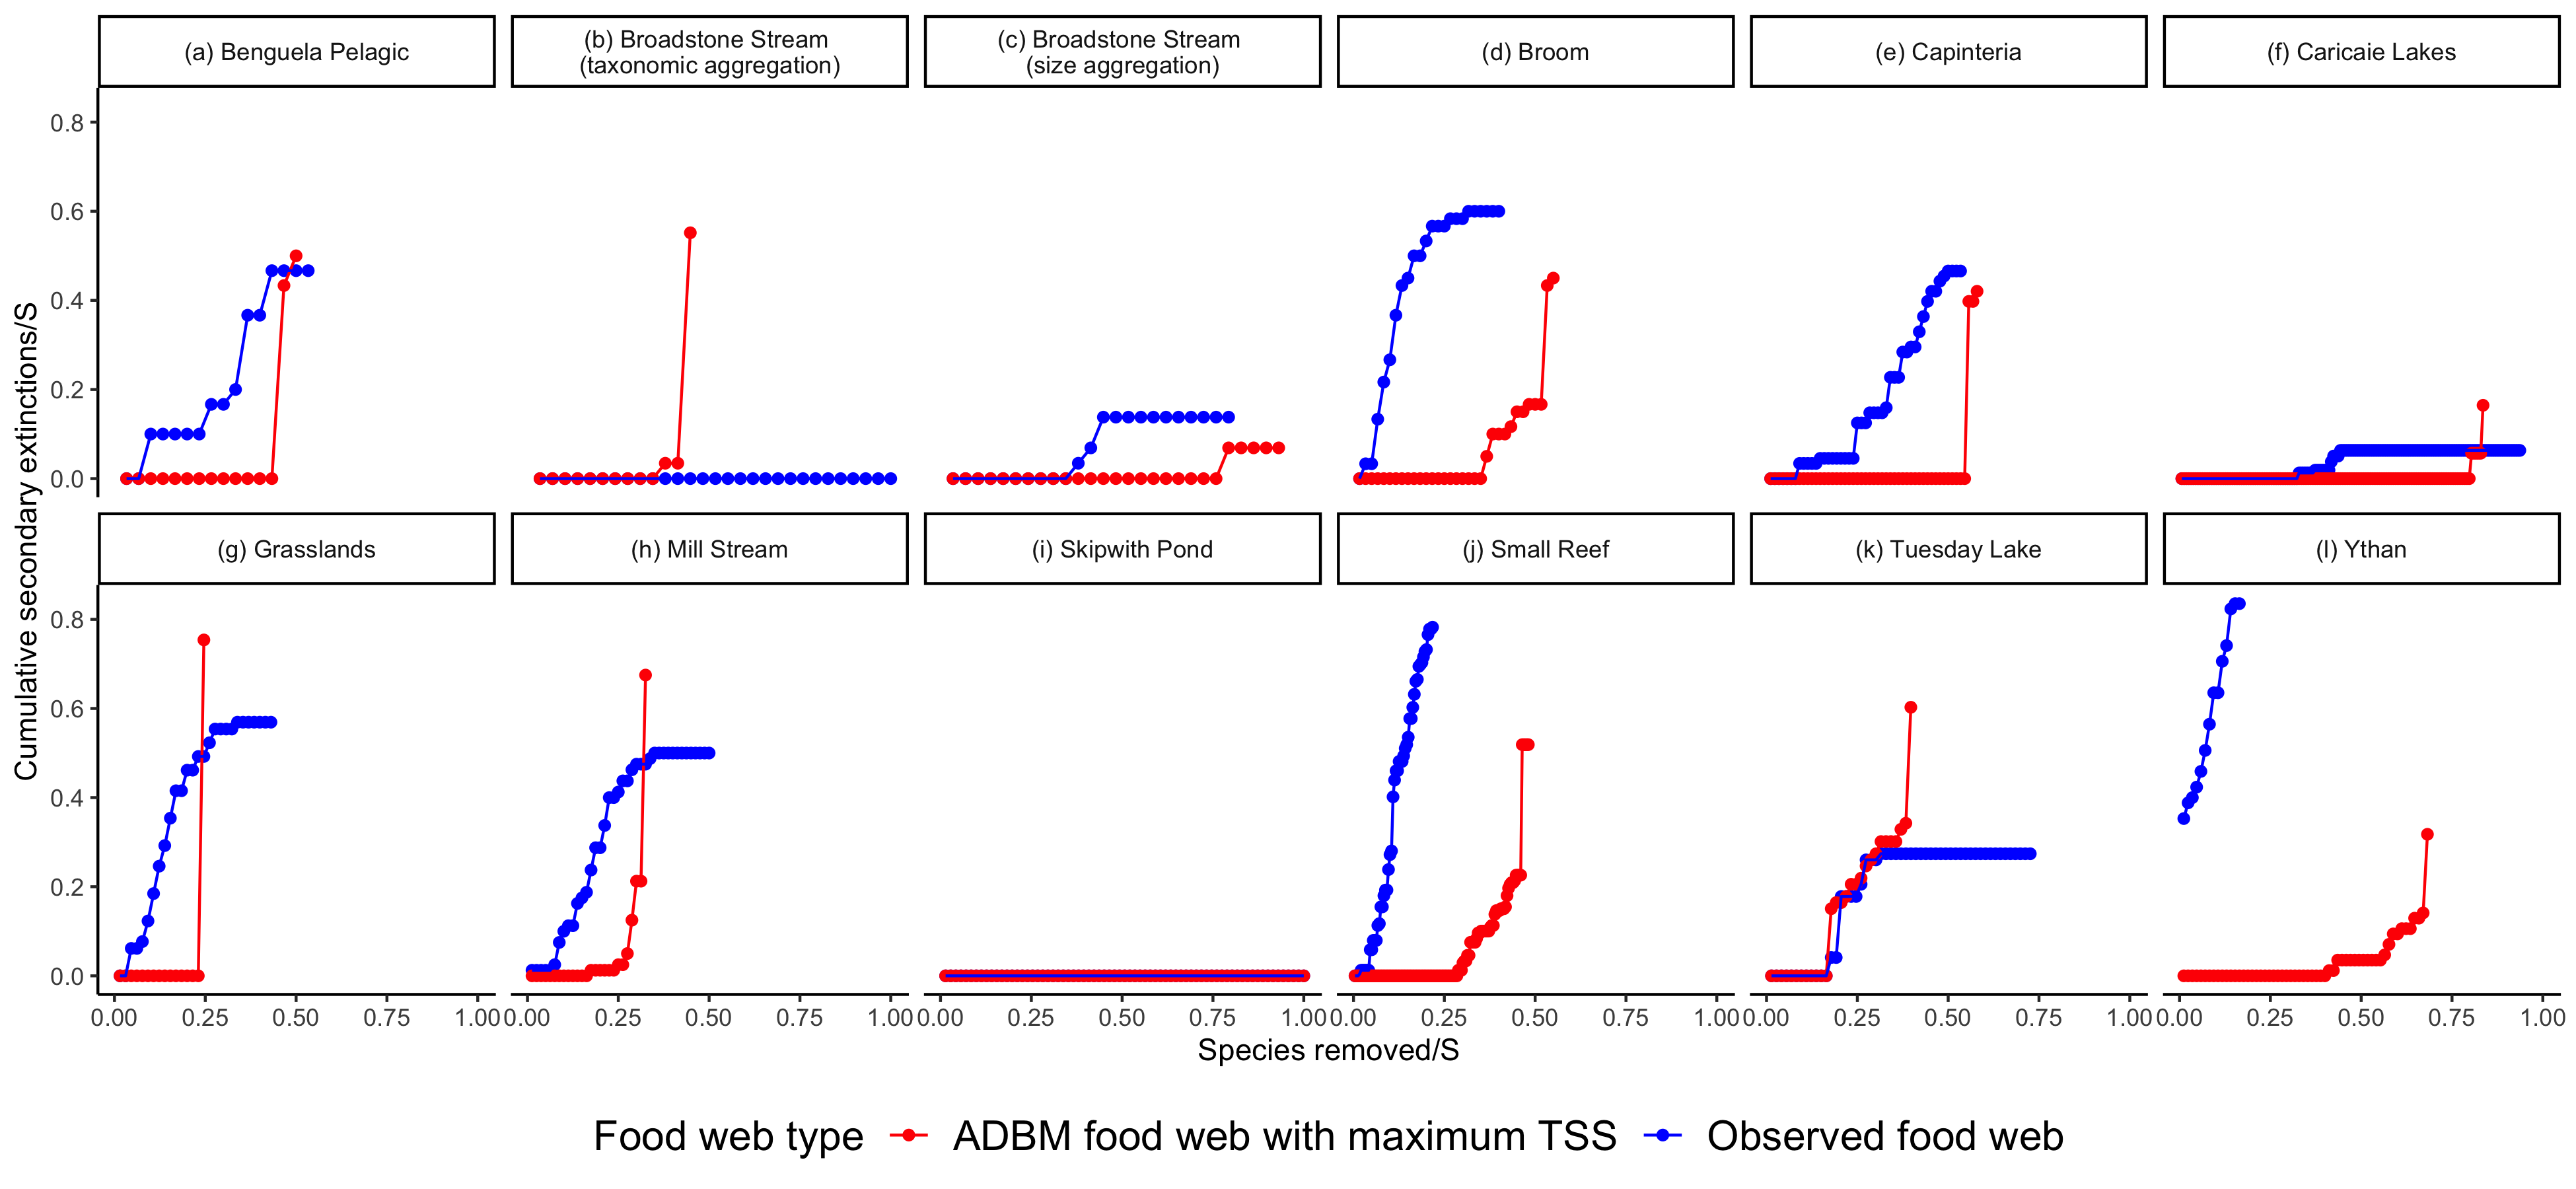
\includegraphics[width=400px]{../results/plot_mostconnected_maxTSS} 

}

\caption{\label{fig:fig_r1} Cumulative secondary extinctions of species resulting from the primary removals of the \textbf{most connected species} in the ADBM predicted food webs corresponding to the maximum TSS and observed food webs. S denotes the number of species in a food web. The cumulative secondary extinctions of species and the number of species removed have been normalised by the number of species.}\label{fig:unnamed-chunk-2}
\end{figure}

In Fig. \ref{fig:fig_r2}, we present the cumulative secondary
extinctions in the ADBM predicted and the observed food webs for five
(out of 1000) independent random extinction sequences to show example
variation caused by different random primary extinction orders. The
secondary extinction curves of the ADBM predicted food webs were steeper
than that of the observed food webs, i.e.~primary removal of some
species in an extinction sequence can lead to the complete collapse of
the remaining food web in the ADBM predicted food webs.

\begin{figure}

{\centering 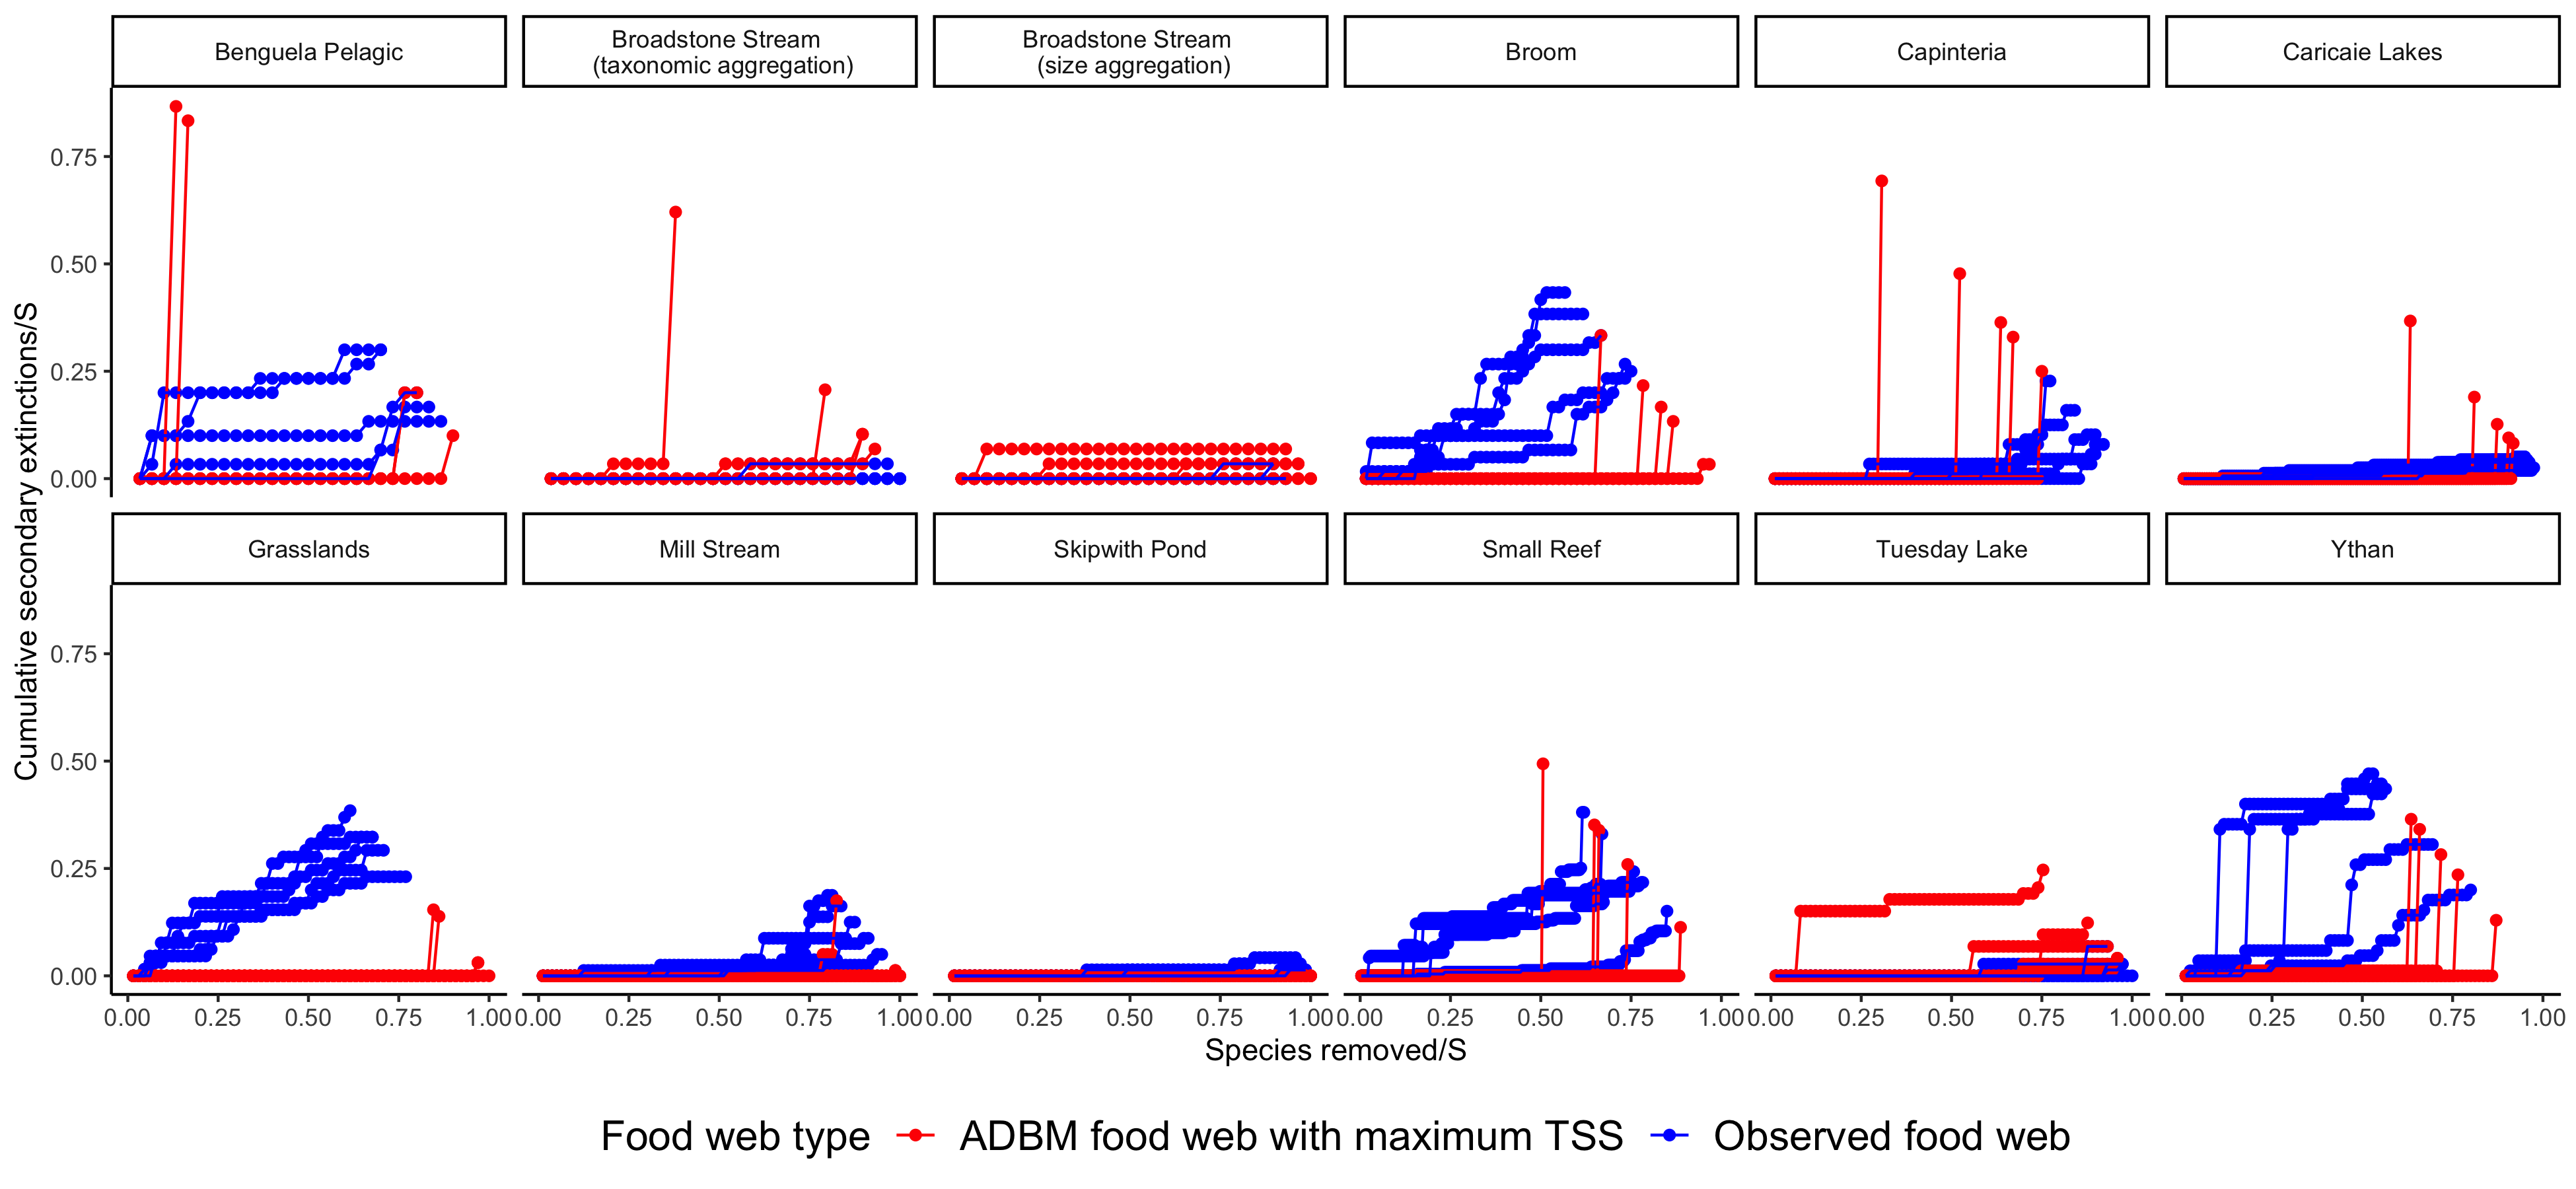
\includegraphics[width=400px]{../results/plot_ra_extlines_maxTSS} 

}

\caption{\label{fig:fig_r2} Cumulative secondary extinctions of species resulting from the primary removals of \textbf{random species} in the ADBM predicted food webs corresponding to the maximum TSS and observed food webs for five (out ot 1000) independent random extinction sequences. S denotes the number of species in a food web. The cumulative secondary extinctions of species and the number of species removed have been normalised by the number of species.}\label{fig:unnamed-chunk-3}
\end{figure}

Compared to the most connected and random extinction scenarios, there
were fewer secondary extinctions in the least connected extinction
scenario, and therefore the secondary extinction curves were flat for
many of the food webs (Fig. \ref{fig:fig_r3}). In some of the food webs,
the extinction curves of the ADBM predicted food webs overlapped with
the observed food webs (Fig. \ref{fig:fig_r3} (b, c, g, h, i, k, l)\}).
In five of the food webs, a very high number of secondary extinctions
occurred at a very low number of primary species removal (Fig.
\ref{fig:fig_r3} (a, d, e, f, j)).

\begin{figure}

{\centering 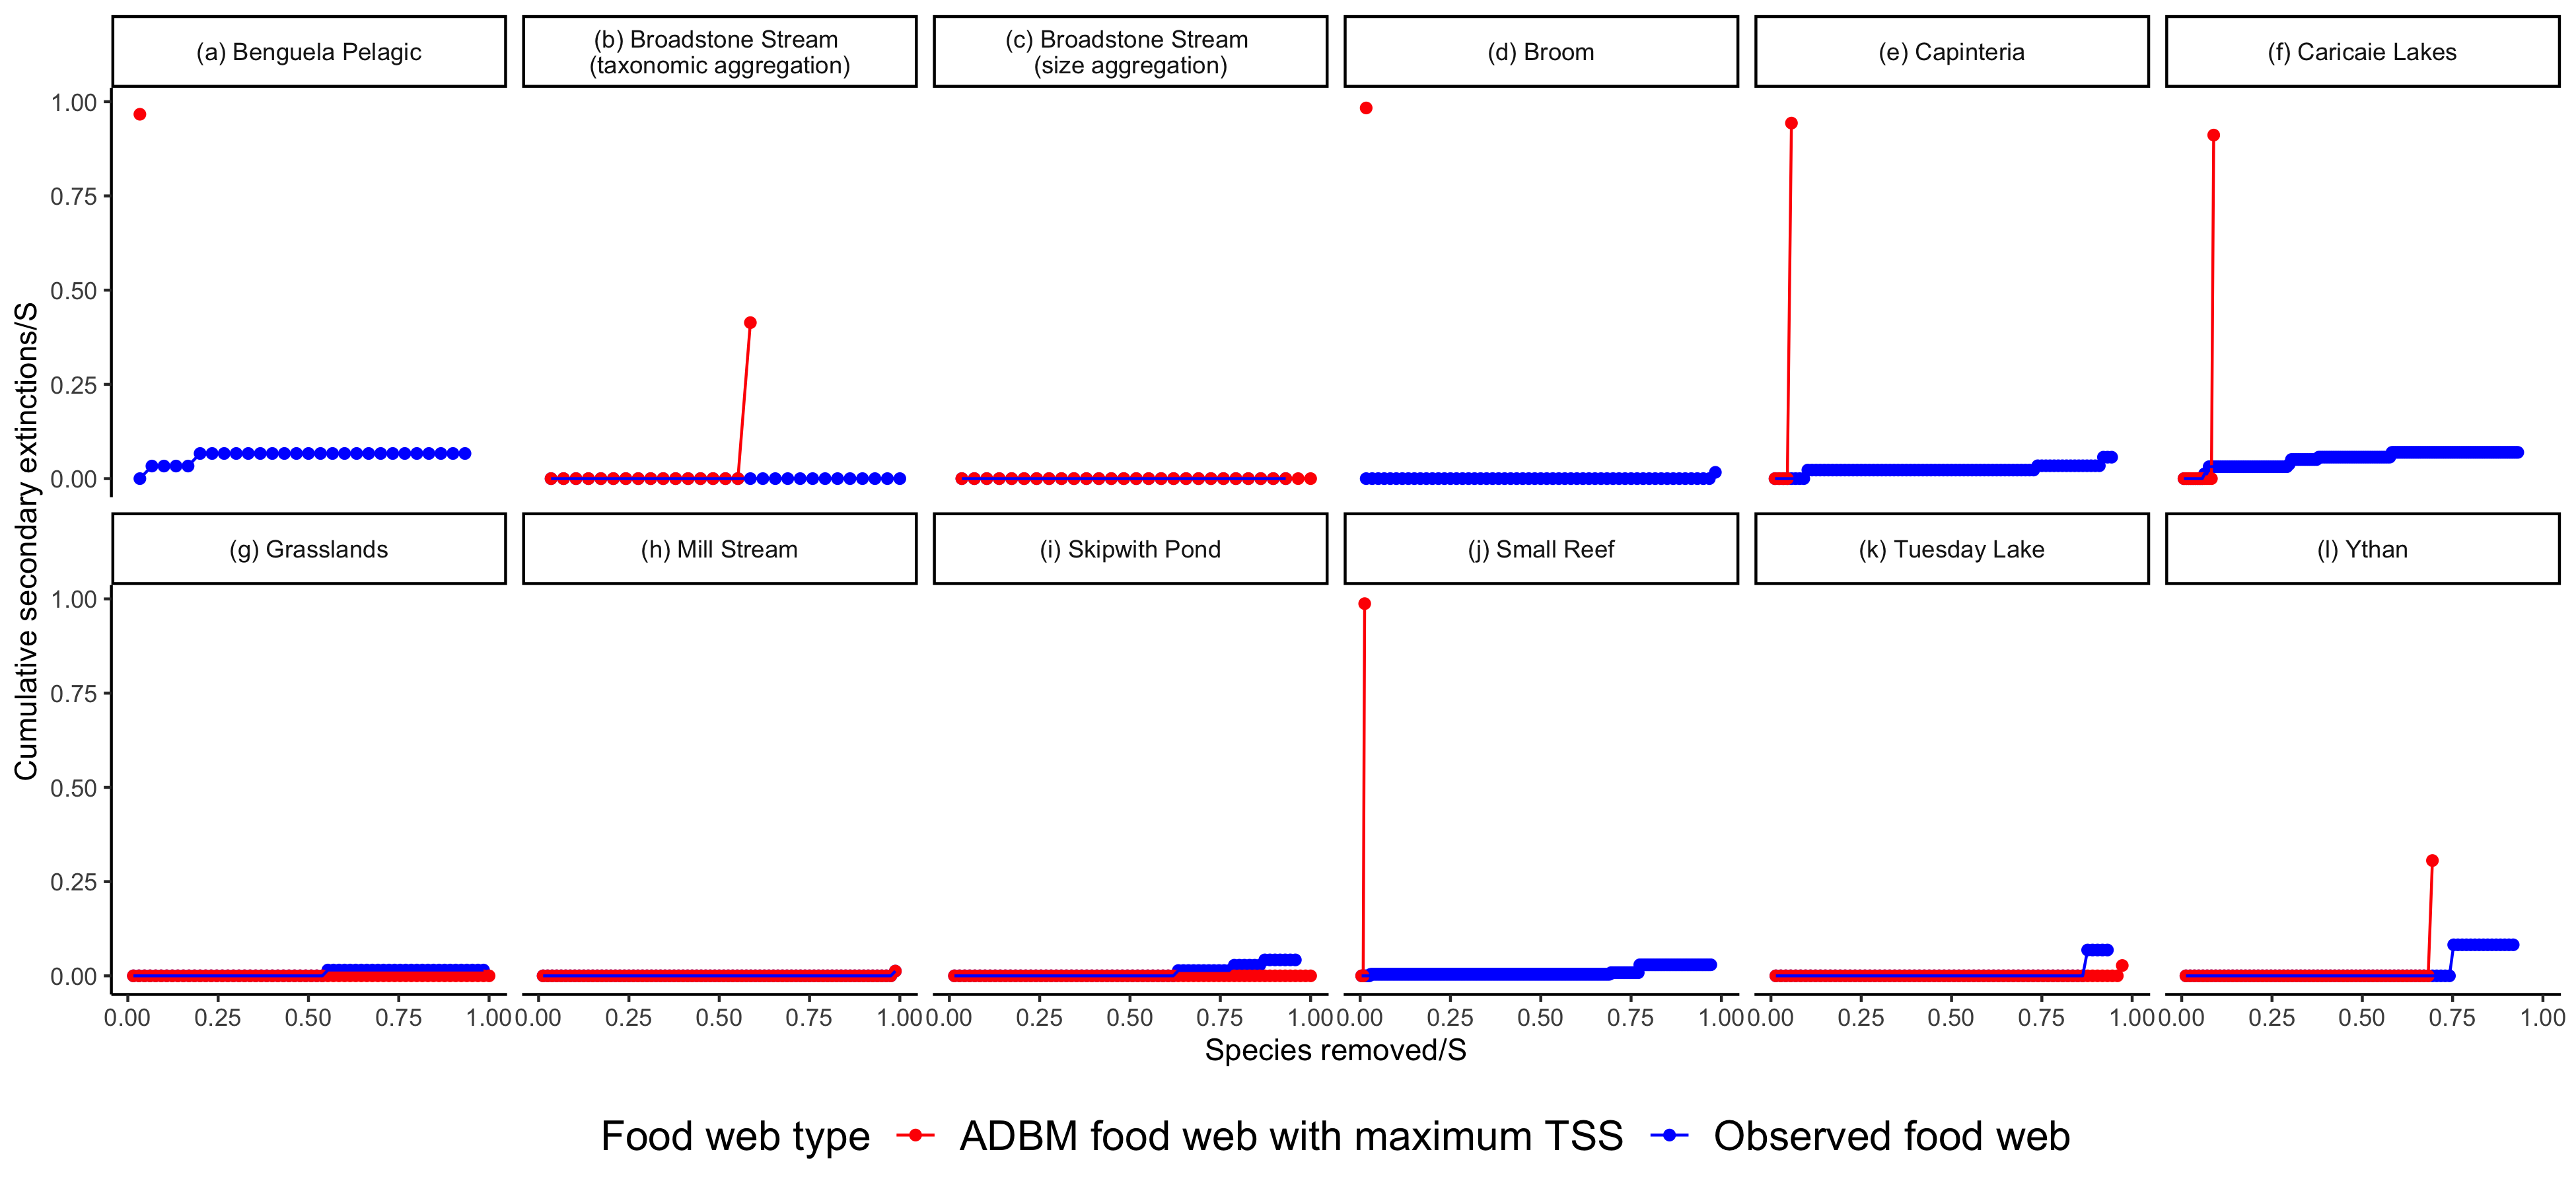
\includegraphics[width=400px]{../results/plot_leastconnected_maxTSS} 

}

\caption{\label{fig:fig_r3} Cumulative secondary extinctions of species resulting from the primary removals of the \textbf{least connected species} in the ADBM predicted food webs corresponding to the maximum TSS and observed food webs. S denotes the number of species in a food web. The cumulative secondary extinctions of species and the number of species removed have been normalised by the number of species.}\label{fig:unnamed-chunk-4}
\end{figure}

\hypertarget{robustness}{%
\subsection{Robustness}\label{robustness}}

The ADBM predicted food webs were more robust than the observed food
webs on average in the most connected and random extinction scenarios
(Fig. \ref{fig:fig_r4} (a, b)). However, there were large variations in
the robustness within the ADBM predicted food webs in the most connected
extinction scenario (Fig. \ref{fig:fig_r4} (a)). For example, the ADBM
predicted Caricaie Lakes food web was more robust than the observed food
web on average but had a larger variation in the robustness within the
ADBM predicted food webs compared to other food webs.

The food webs were more robust to the random extinction scenario than
the most connected scenario (Fig. \ref{fig:fig_r4} (a, b)). Small Reef
and Benguela Pelagic food webs had more variations in robustness within
the ADBM predicted food webs as compared to the other food webs (Fig.
\ref{fig:fig_r4} (b)). Skipwith Pond, Broadstone Stream (taxonomic
aggregation) and Broadstone Stream (size aggregation) food webs were the
most robust (Median \(R_{50} = 0.5\)) for both ADBM predicted and
observed food webs. Although there were few less robust ADBM predicted
food webs in the Broadstone Stream (size aggregation) as shown by the
outliers. The food webs were more robust to the random extinction
scenario than the most connected scenario (Fig. \ref{fig:fig_r4} (a,
b)). Small Reef and Benguela Pelagic food webs had more variations in
robustness within the ADBM predicted food webs as compared to the other
food webs (Fig. \ref{fig:fig_r4} (b)). Skipwith Pond, Broadstone Stream
(taxonomic aggregation) and Broadstone Stream (size aggregation) food
webs were the most robust (Median \(R_{50} = 0.5\)) for both ADBM
predicted and observed food webs. Although there were few less robust
ADBM predicted food webs in the Broadstone Stream (size aggregation) as
shown by the outliers.

In the least connected extinction scenario, the food webs had a very
high robustness (Median \(R_{50} = 0.5\)) for most of the food webs
(Fig. \ref{fig:fig_r4} (c)), however there were some exceptions. The
ADBM predicted food webs for Small Reef and Benguela Pelagic had very
low median robustness. Benguela Pelagic, Broom and Capinteria food webs
from the ADBM had larger variations in robustness when compared to that
of the others.

\begin{figure}

{\centering 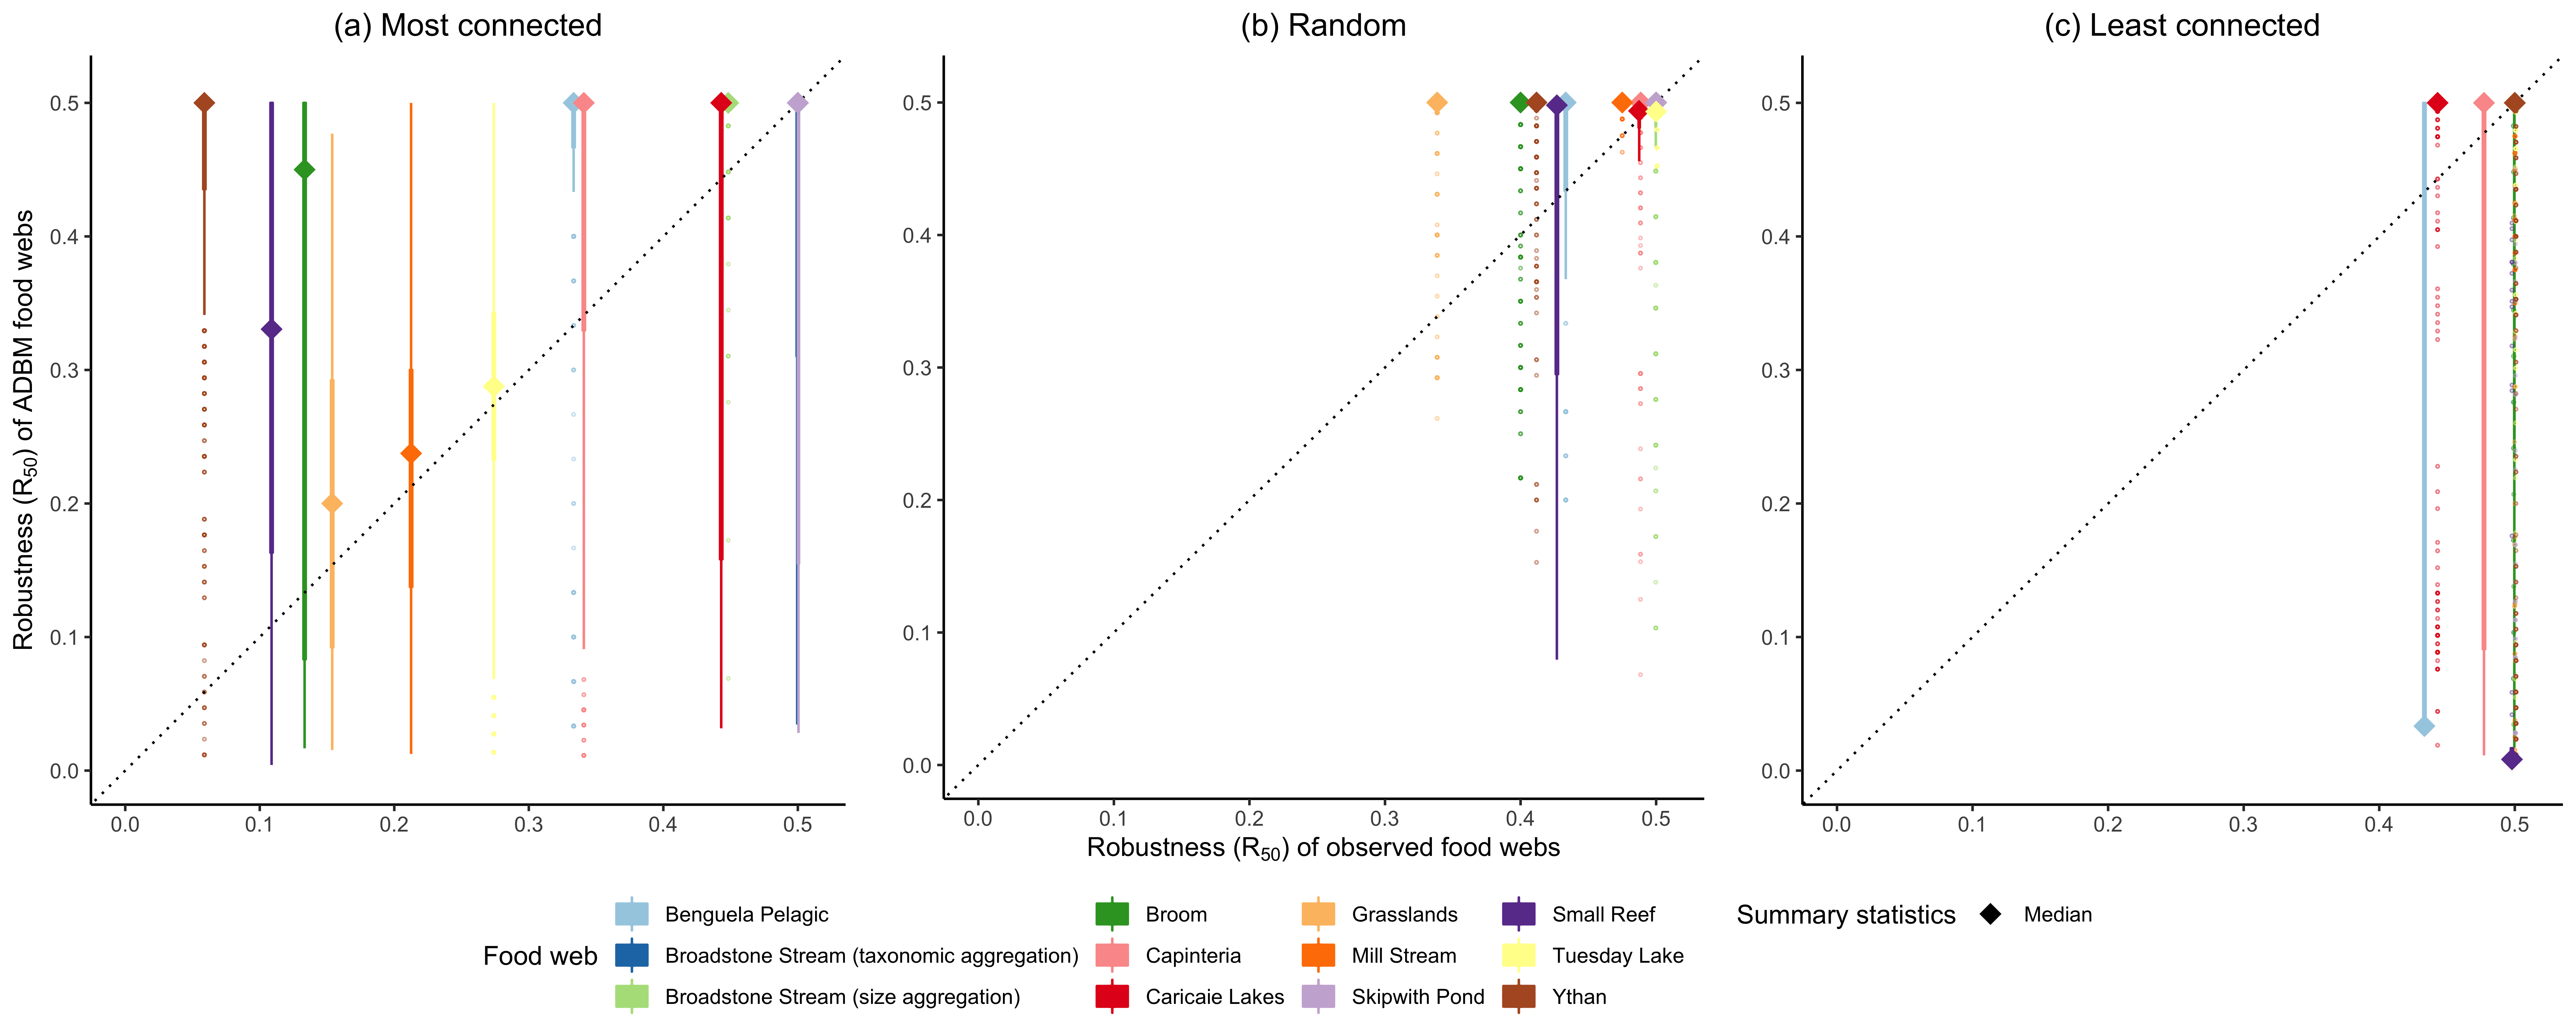
\includegraphics[width=450px]{../results/plot_R50_ADBM_vs_obs} 

}

\caption{\label{fig:fig_r4} Robustness comparison between the ADBM predicted food webs and the observed food webs for 12 food webs across different ecosystems. Here, $R_{50}$ is the proportion of species that have to be removed to achieve a total loss of at least 50\% of total species (primary removals and secondary extinctions). Box represent the 25th and 75th percentile; solid diamond represents the median; whisker represents outlier limits; the outlier coefficient used was 1.5. Some points are not visible due to perfect overlap in b and c. Refer to Fig. 7 in the Supplementary Information for a faceted visualisation. The dashed black lines are the 1:1 relationships for reference.}\label{fig:unnamed-chunk-5}
\end{figure}

In all of the food webs except Small Reef and Broadstone Stream
(taxonomic aggregation), the effect size of connectance on robustness
was positive on average in the most connected extinction scenario (Fig.
\ref{fig:fig_r5} (a)), i.e.~greater connectance had a positive effect on
the robustness. In the random extinction scenario, there was a positive
effect of greater connectance on the robustness for Ythan, Small Reef,
Mill Stream, Grasslands, Caricaie Lakes, Capinteria, Broom and Benguela
Pelagic (Fig. \ref{fig:fig_r5} (b)). However, the effect size varied
across the food webs. In the least connected extinction scenario, the
median effect sizes were zero or very close to zero for all the food
webs except Benguela Pelagic and Small Reef food webs where the median
effect sizes were negative (Fig. \ref{fig:fig_r5} (c)). However, there
were lots of outlier effect sizes less than zero.

\begin{figure}

{\centering 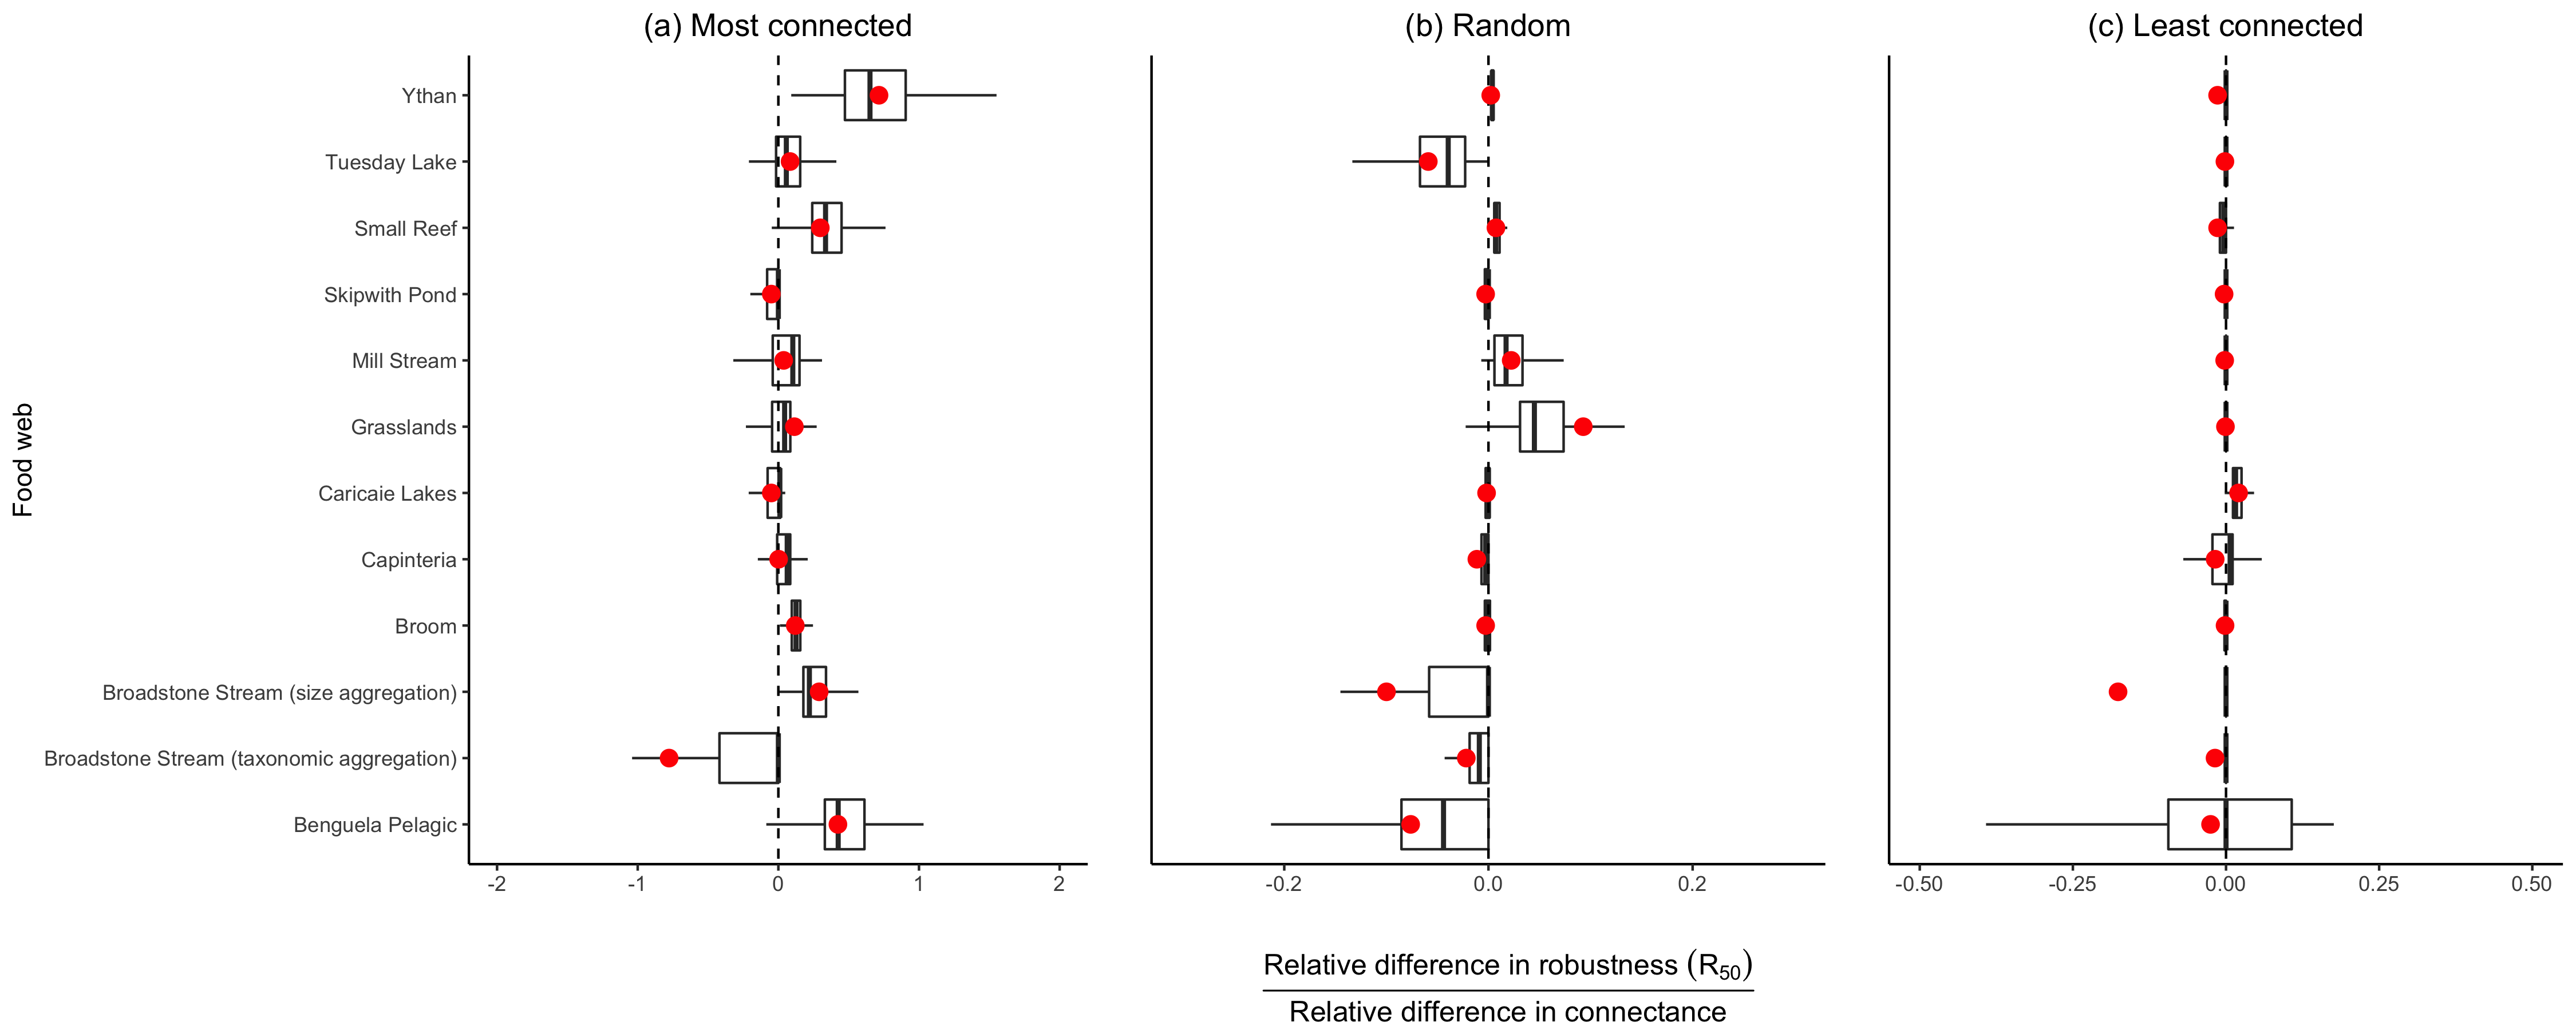
\includegraphics[width=450px]{../results/plot_R50_slope} 

}

\caption{\label{fig:fig_r5} Effect size (i.e. ratio of the difference in normalised robustness between ADBM predicted food webs and observed food webs to the difference in their normalised connectance) shown for the 12 food webs. Box represent the 25th and 75th percentile; bold black midline represents the median; whisker represents outlier limits; the outlier coefficient used was 1.5.}\label{fig:unnamed-chunk-6}
\end{figure}

\hypertarget{discussion}{%
\section{Discussion}\label{discussion}}

As expected, the ADBM predicted food webs were more robust than the
observed food webs on average. The considerable variation of the
robustness of the ADBM predicted food webs suggests, however, that
undersampling in food webs can lead to considerable uncertainty in the
estimates of food web robustness, even when a model is used to
compensate for undersampling. Furthermore, as was previously found, the
food webs are least robust to primary extinction of the most connected
species compared to that of least connected and random extinction
scenarios on average. Future development would be to understand how
undersampling, i.e.~predicted greater connectance, influences the
stability of the dynamics of the ADBM predicted food webs against that
of the observed food webs and compare it with the patterns in our study
in which extinction occur only by topological criteria. However, one
would expect a decrease in food web stability with greater connectance
(Martinez et al., 2006; May, 1972).

As mentioned, the robustness of the ADBM predicted food webs was higher
than that of the observed food webs on average (Fig. \ref{fig:fig_r4})
for all of the 12 food web ecosystems (with some exceptions). This is
likely due to the greater connectance of the ADBM predicted food webs as
compared to that of the observed food webs because a species in a food
web with a higher connectance has, on average, more trophic links as
compared to a food web with a lower connectance (Fig. \ref{fig:fig_r5}).
Our study suggests that it is important to consider undersampling in
observed food webs when computing their robustness.

Contrary to general expectations (Dunne et al., 2002b), food web
robustness did not always increase with the connectance (Fig.
\ref{fig:fig_r5}). For example, the Benguela Pelagic and Small Reef ADBM
predicted food webs were surprisingly less robust to primary extinctions
on average in the least connected extinction scenario compared to the
observed food webs (Fig. \ref{fig:fig_r4} (c) and \ref{fig:fig_r5} (c)).
In these two food webs, the extinction of the least connected species
could cause an almost complete, or complete collapse of the food web. We
suspect this is because the ADBM predicted food webs have a lower
proportion of basal species when compared to that of the observed food
webs (Fig: 6 (a) in Gupta et al. (2022)). As a result, these low-degree
basal species are the ones to be removed at an early stage in the
deletion sequence, thereby resulting in an earlier food web collapse in
the ADBM predicted food web as compared to that of the observed food web
(Fig: \ref{fig:fig_r3} (a) and (j)). This suggests that the greater
connectance predicted by the ADBM resulted in a more robust food web on
average. However, differences in the predicted food web properties, such
as a lower proportion of basal species and higher maximum trophic level
(Fig: \ref{fig:fig_a1}) when compared to that of the predicted food webs
counteracted that effect and led to reduced robustness. On average, a
consumer in a food web with a higher maximum trophic level would have
fewer resources and be more susceptible to extinction than a consumer in
a food web with a lower maximum trophic level (Binzer et al., 2011).
This suggests that food web properties other than connectance play an
important role in determining a food web's robustness and, therefore,
should also be taken into account (Binzer et al., 2011; Mendonça et al.,
2022; Riede et al., 2011).

As with any food web model, we expect that there are real false
positives in the food webs predicted by the ADBM. Real false positive
means that the food web model predicts a link between two species that
can never interact. (The other type of false positive is when the model
predicts a link that was not observed but could have been observed if
the food web was sampled enough. In this case, further sampling should
result in the link being observed and a change from false positive to
true positive.) Firstly, this may be because the ADBM uses only body
size as a trait. A trait uncorrelated with the body size may be
influential in determining the interaction between two species (Gupta et
al., 2022). Secondly, the ADBM can only predict diets that are
contiguous with respect to the size of the prey. I.e. it cannot predict
that the consumer will consume prey of size 1 and 3, and not consume
prey of size 2. However, it is important to note that observed diets are
not always contiguous when prey are ordered by their size due to some
ecological differences in how predator species choose their prey (Caron
et al., 2022). Hence, it would be intriguing to extend our study to use
other food web models based on size-based rules, such as Gravel et al.
(2013) and Vagnon et al. (2021), to understand if the results are
dependent on the decision of model selection. We expect to get a similar
result in a size-based deterministic model but a different result,
i.e.~lower robustness in a size-based stochastic model as compared to
the ADBM because the latter can take into account non-contiguity in
predator diets (Williams et al., 2010). It would also be interesting to
use food web models not based on body size, such as Cattin et al. (2004)
and Allesina et al. (2008). We expect to have a difference in results
based on whether the trophic interactions in the food webs are governed
by size-structured rules or not.

It would be intriguing to know if this difference in connectance has a
similar influence on the dynamical stability of the food webs as well.
Hence, a prospect could be to use a dynamical model (for example, the
bioenergetic food web model by Brose et al. (2006)) to model the
temporal dynamics of the ADBM predicted food webs. We expect that the
greater connectance will lead to reduced dynamical stability in the ADBM
predicted food web compared to that of the predicted food web. The
difference in stability will be linearly related to the difference in
connectance because Martinez et al. (2006) has shown that food web
stability linearly decreases with connectance.

Since the ADBM predicted food webs have a lower proportion of basal
species and a higher maximum trophic level as compared to that of the
observed food webs (Fig: 6 (a) in Gupta et al. (2022) and Fig.
\ref{fig:fig_a1} in Supplementary Information), it would be interesting
to use these properties as summary statistics to parameterise the ADBM
and investigate how that influences the difference in the robustness
between the ADBM predicted and the observed food webs. We would expect a
more highly constrained predicted food web structure, lower variation in
robustness, and a greater apparent influence of connectance on
robustness.

We have used a food web model to compensate for undersampling in
recorded food webs and thereby quantified the influence of missing
links, i.e.~greater connectance on the topological robustness of 12 food
webs from various ecosystems. We found that the greater connectance can
have a large impact on the robustness of the food webs while at the same
time producing large variations in robustness among the predicted food
webs. Furthermore, differences in other structural food web properties
between the ADBM predicted food webs and the observed food webs are also
responsible.

\hypertarget{acknowledgements}{%
\section{Acknowledgements}\label{acknowledgements}}

This work was supported by the University Research Priority Program
Global Change and Biodiversity (Grant number: U-704-04-11) of the
University of Zurich. We thank the Petchey group members for their
valuable suggestions in the manuscript.

\hypertarget{conflict-of-interest}{%
\section{Conflict of interest}\label{conflict-of-interest}}

None declared

\hypertarget{author-contributions}{%
\section{Author contributions}\label{author-contributions}}

\textbf{Anubhav Gupta:} Conceptualisation; Data curation; Formal
analysis; Investigation; Methodology; Project administration; Software;
Validation; Writing -- original draft; Writing -- review and editing.
\textbf{Owen L. Petchey:} Conceptualization; Funding acquisition;
Resources; Supervision; Writing -- review \& editing.

\hypertarget{data-accessibility-statement}{%
\section{Data Accessibility
Statement}\label{data-accessibility-statement}}

All the data used in this study was collected in other studies and is
openly available. We list those studies and the open access source in
Table \ref{fig:tab_1}. The complete code used in the analysis is
available in the repository
\url{https://doi.org/10.5281/zenodo.7180835}.

\hypertarget{supplementary-information}{%
\section{Supplementary Information}\label{supplementary-information}}

\begin{figure}[H]

{\centering 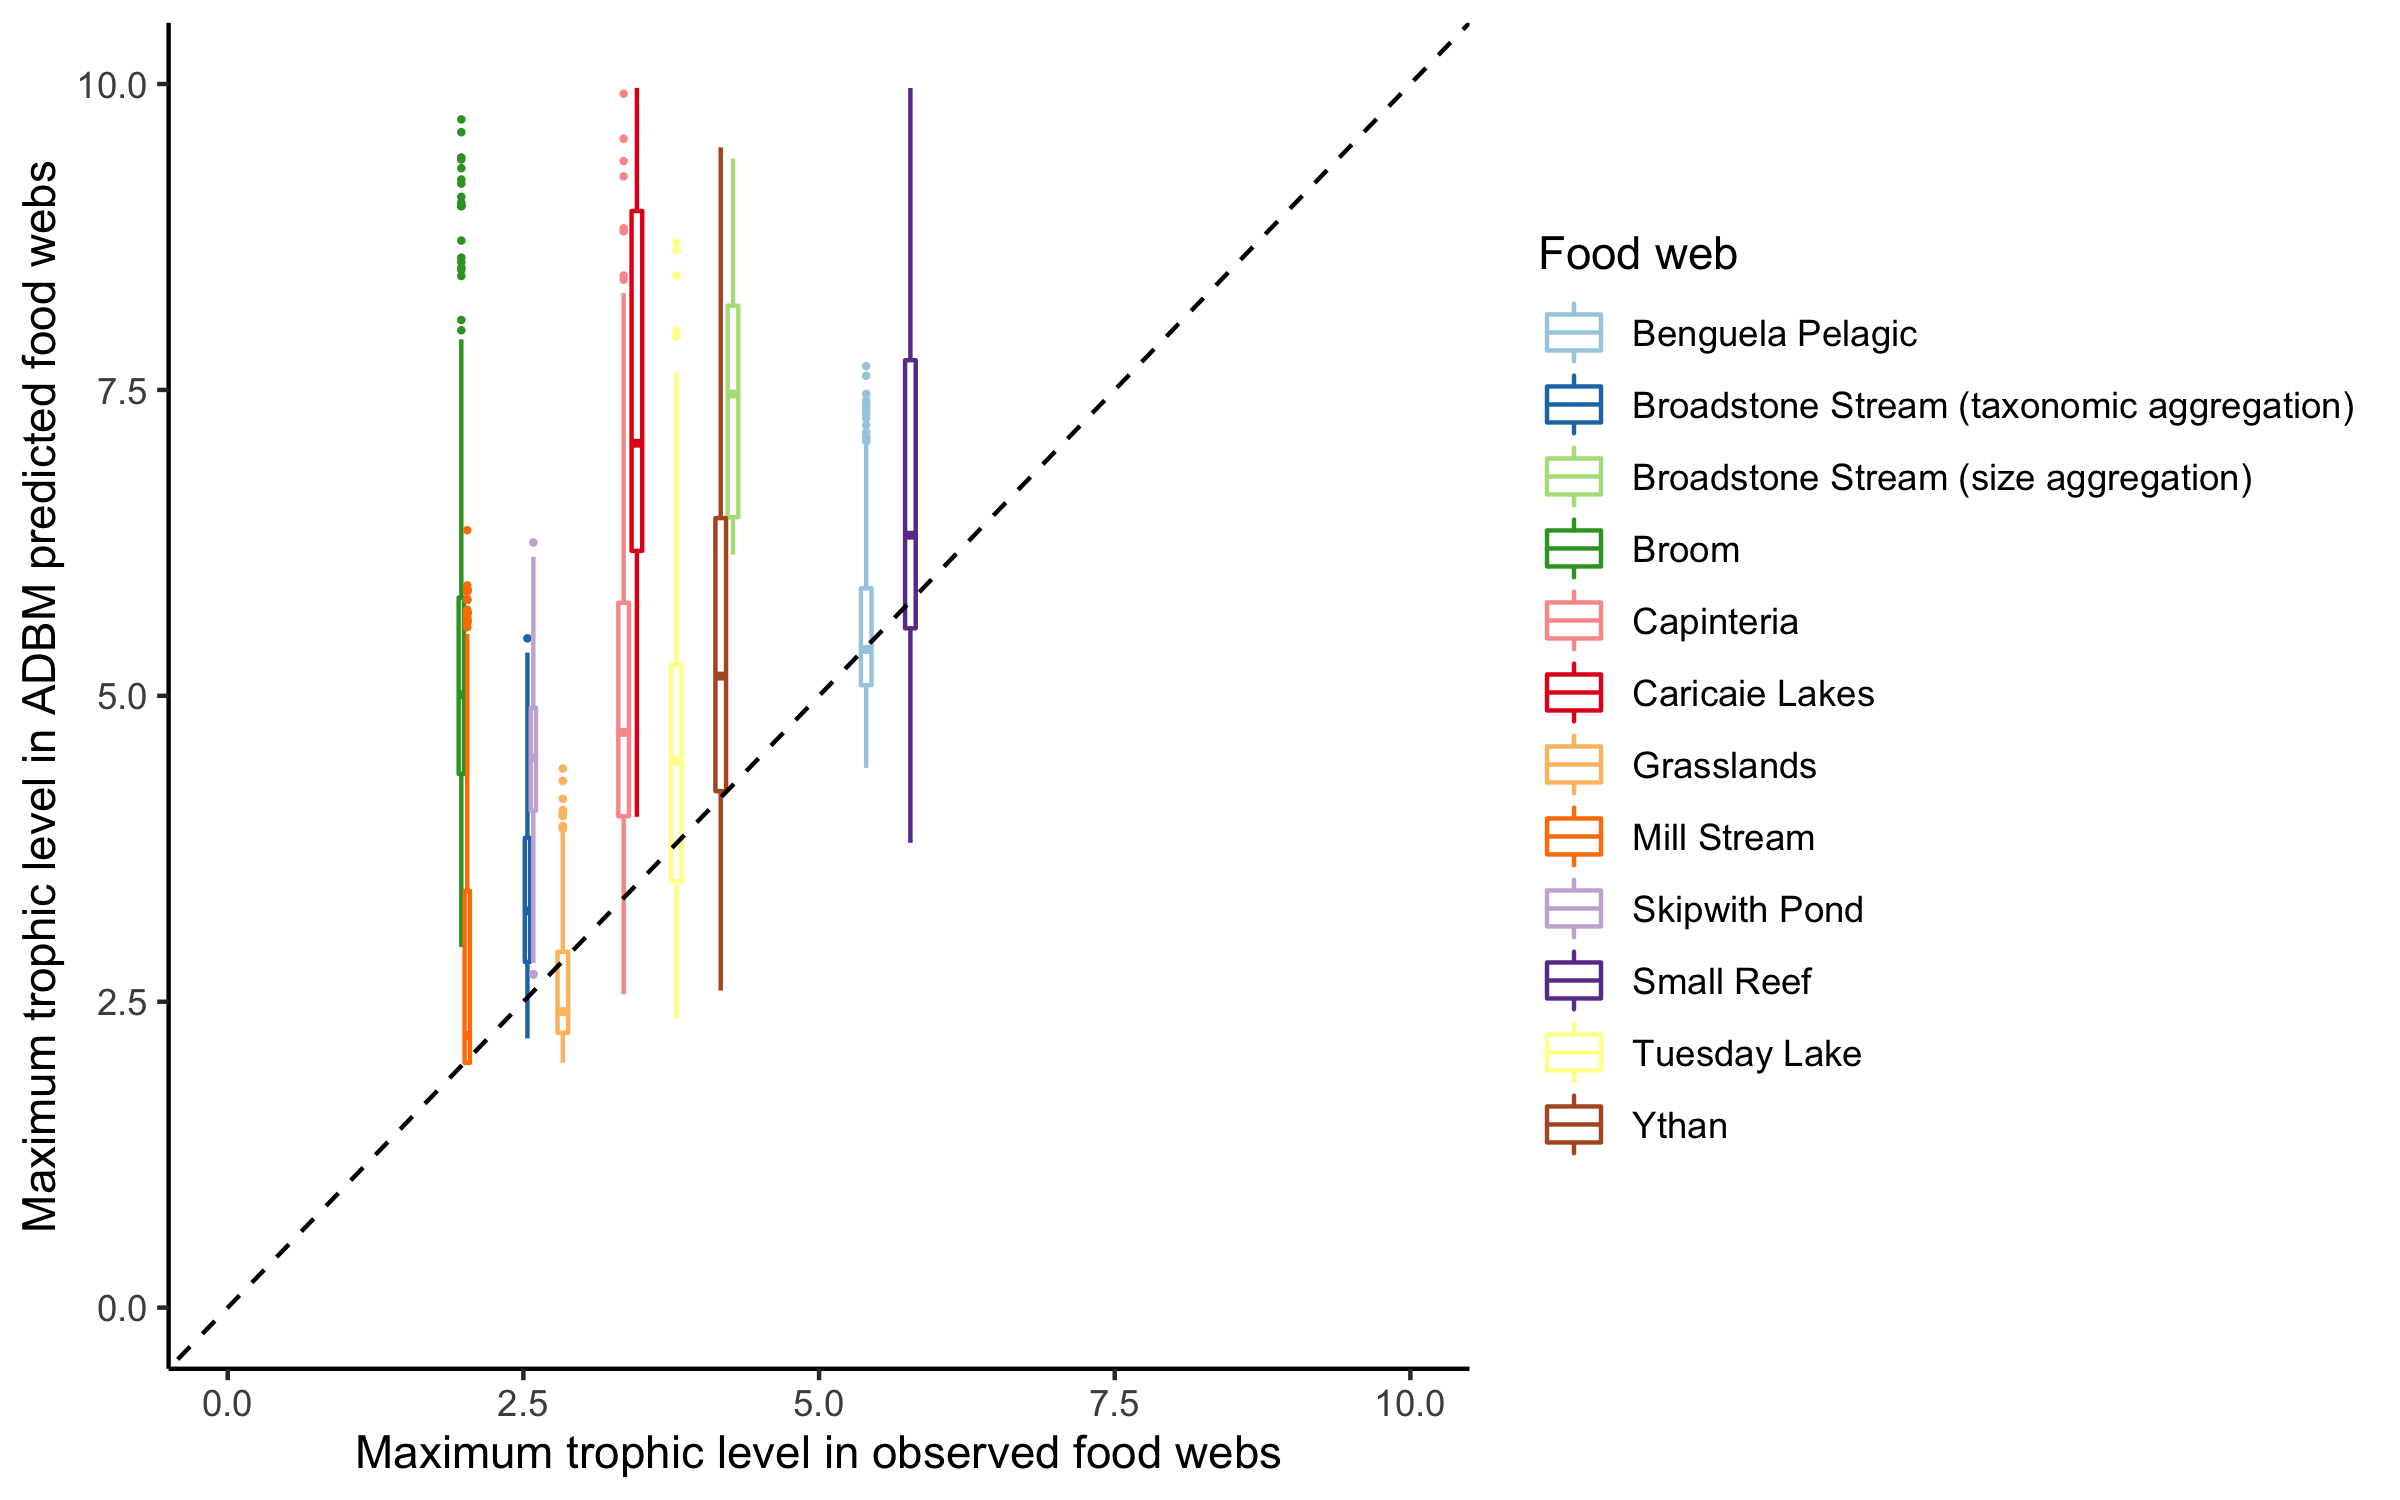
\includegraphics[width=450px]{../results/plot_max_tl_ADBM_vs_emp} 

}

\caption{\label{fig:fig_a1} The maximum trophic level of ADBM predicted food webs plotted against that of the observed food webs. Box represent the 25th and 75th percentile; bold midline represents the median; whisker represents outlier limits; the outlier coefficient used was 1.5. The dashed black lines are the 1:1 relationships for reference.}\label{fig:unnamed-chunk-7}
\end{figure}

\begin{figure}[H]

{\centering 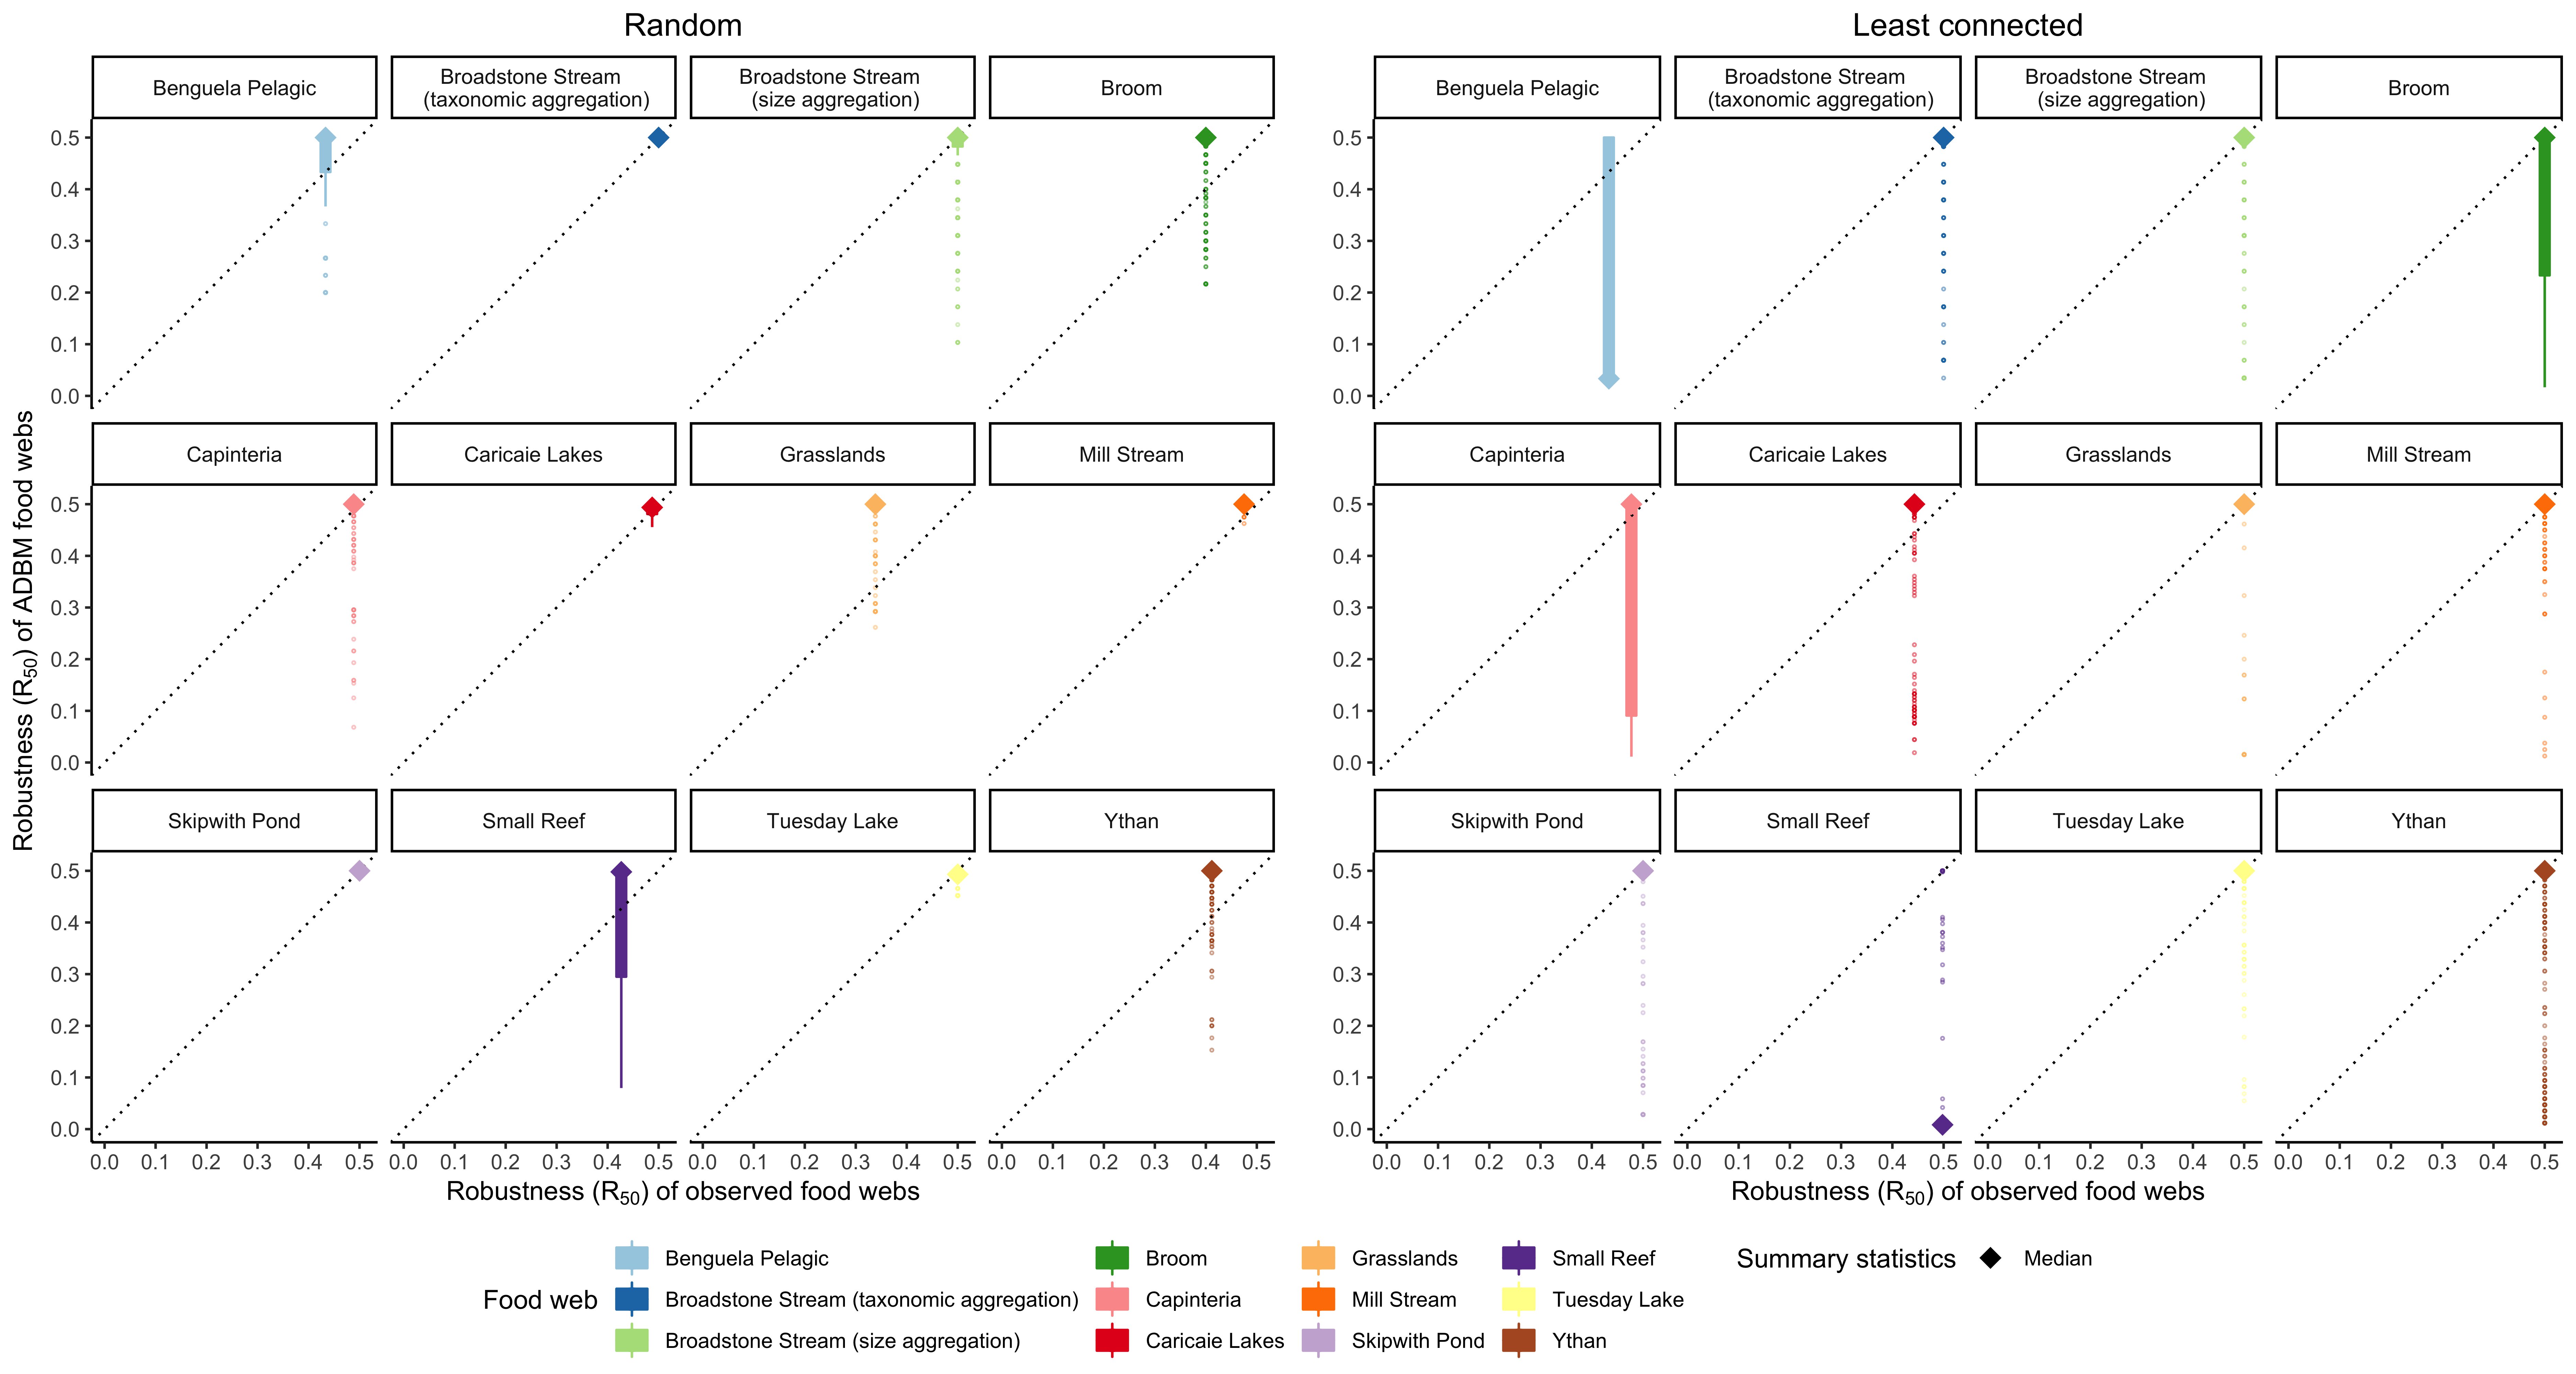
\includegraphics[width=450px]{../results/plot_R50_ADBM_vs_obs_ra_lc_facet} 

}

\caption{\label{fig:fig_a2} Robustness comparison between the ADBM predicted food webs and the observed food webs for 12 food webs across different ecosystems for random and least connected extinction scenarios. Here, $R_{50}$ is the proportion of species that have to be removed to achieve a total loss of at least 50\% of total species (primary removals and secondary extinctions). Box represent the 25th and 75th percentile; solid diamond represents the median; whisker represents outlier limits; the outlier coefficient used was 1.5. The dashed black lines are the 1:1 relationships for reference.}\label{fig:unnamed-chunk-8}
\end{figure}

\hypertarget{references}{%
\section*{References}\label{references}}
\addcontentsline{toc}{section}{References}

\hypertarget{refs}{}
\begin{CSLReferences}{1}{0}
\leavevmode\vadjust pre{\hypertarget{ref-albertStatisticalMechanicsComplex2002}{}}%
Albert, R., \& Barab'asi, A.-L. (2002). Statistical mechanics of complex
networks. \emph{Reviews of Modern Physics}, \emph{74}(1), 47--97.
\url{https://doi.org/10.1103/RevModPhys.74.47}

\leavevmode\vadjust pre{\hypertarget{ref-allesinaGeneralModelFood2008}{}}%
Allesina, S., Alonso, D., \& Pascual, M. (2008). A {General Model} for
{Food Web Structure}. \emph{Science}, \emph{320}(5876), 658--661.
\url{https://doi.org/10.1126/science.1156269}

\leavevmode\vadjust pre{\hypertarget{ref-bergUsingSensitivityAnalysis2011}{}}%
Berg, S., Christianou, M., Jonsson, T., \& Ebenman, B. (2011). Using
sensitivity analysis to identify keystone species and keystone links in
size-based food webs. \emph{Oikos}, \emph{120}(4), 510--519.
\url{https://doi.org/10.1111/j.1600-0706.2010.18864.x}

\leavevmode\vadjust pre{\hypertarget{ref-binzerSusceptibilitySpeciesExtinctions2011}{}}%
Binzer, A., Brose, U., Curtsdotter, A., Eklöf, A., Rall, B. C., Riede,
J. O., \& de Castro, F. (2011). The susceptibility of species to
extinctions in model communities. \emph{Basic and Applied Ecology},
\emph{12}(7), 590--599. \url{https://doi.org/10.1016/j.baae.2011.09.002}

\leavevmode\vadjust pre{\hypertarget{ref-broseAllometricScalingEnhances2006}{}}%
Brose, U., Williams, R. J., \& Martinez, N. D. (2006). Allometric
scaling enhances stability in complex food webs. \emph{Ecology Letters},
\emph{9}(11), 1228--1236.
\url{https://doi.org/10.1111/j.1461-0248.2006.00978.x}

\leavevmode\vadjust pre{\hypertarget{ref-caronAddressingEltonianShortfall}{}}%
Caron, D., Maiorano, L., Thuiller, W., \& Pollock, L. J. (2022).
Addressing the {Eltonian} shortfall with trait-based interaction models.
\emph{Ecology Letters}, \emph{n/a}(n/a).
\url{https://doi.org/10.1111/ele.13966}

\leavevmode\vadjust pre{\hypertarget{ref-cattinPhylogeneticConstraintsAdaptation2004}{}}%
Cattin, M.-F., Bersier, L.-F., Banašek-Richter, C., Baltensperger, R.,
\& Gabriel, J.-P. (2004). Phylogenetic constraints and adaptation
explain food-web structure. \emph{Nature}, \emph{427}(6977, 6977),
835--839. \url{https://doi.org/10.1038/nature02327}

\leavevmode\vadjust pre{\hypertarget{ref-davidImpactsInvasiveSpecies2017}{}}%
David, P., Th'ebault, E., Anneville, O., Duyck, P.-F., Chapuis, E., \&
Loeuille, N. (2017). Impacts of {Invasive Species} on {Food Webs}. In
\emph{Advances in {Ecological Research}} (Vol. 56, pp. 1--60).
{Elsevier}. \url{https://doi.org/10.1016/bs.aecr.2016.10.001}

\leavevmode\vadjust pre{\hypertarget{ref-dunneCascadingExtinctionsCommunity2009}{}}%
Dunne, J. A., \& Williams, R. J. (2009). Cascading extinctions and
community collapse in model food webs. \emph{Philosophical Transactions
of the Royal Society B: Biological Sciences}, \emph{364}(1524),
1711--1723. \url{https://doi.org/10.1098/rstb.2008.0219}

\leavevmode\vadjust pre{\hypertarget{ref-dunne2002network}{}}%
Dunne, J. A., Williams, R. J., \& Martinez, N. D. (2002a). Network
structure and biodiversity loss in food webs: Robustness increases with
connectance. \emph{Ecology Letters}, \emph{5}(4), 558--567.

\leavevmode\vadjust pre{\hypertarget{ref-dunneNetworkStructureBiodiversity2002}{}}%
Dunne, J. A., Williams, R. J., \& Martinez, N. D. (2002b). Network
structure and biodiversity loss in food webs: Robustness increases with
connectance. \emph{Ecology Letters}, \emph{5}(4), 558--567.
\url{https://doi.org/10.1046/j.1461-0248.2002.00354.x}

\leavevmode\vadjust pre{\hypertarget{ref-dunne2004}{}}%
Dunne, J., Williams, R., \& Martinez, N. (2004). Network structure and
robustness of marine food webs. \emph{Marine Ecology Progress Series},
\emph{273}, 291--302. \url{https://doi.org/10.3354/meps273291}

\leavevmode\vadjust pre{\hypertarget{ref-ebenmanUsingCommunityViability2005}{}}%
Ebenman, B., \& Jonsson, T. (2005). Using community viability analysis
to identify fragile systems and keystone species. \emph{Trends in
Ecology \& Evolution}, \emph{20}(10), 568--575.
\url{https://doi.org/10.1016/j.tree.2005.06.011}

\leavevmode\vadjust pre{\hypertarget{ref-ebenmanCOMMUNITYVIABILITYANALYSIS2004}{}}%
Ebenman, B., Law, R., \& Borrvall, C. (2004). {COMMUNITY VIABILITY
ANALYSIS}: {THE RESPONSE OF ECOLOGICAL COMMUNITIES TO SPECIES LOSS}.
\emph{Ecology}, \emph{85}(9), 2591--2600.
\url{https://doi.org/10.1890/03-8018}

\leavevmode\vadjust pre{\hypertarget{ref-gravelInferringFoodWeb2013a}{}}%
Gravel, D., Poisot, T., Albouy, C., Velez, L., \& Mouillot, D. (2013).
Inferring food web structure from predator--prey body size
relationships. \emph{Methods in Ecology and Evolution}, \emph{4}(11),
1083--1090. \url{https://doi.org/10.1111/2041-210X.12103}

\leavevmode\vadjust pre{\hypertarget{ref-guptaSimultaneouslyEstimatingFood2022}{}}%
Gupta, A., Furrer, R., \& Petchey, O. L. (2022). Simultaneously
estimating food web connectance and structure with uncertainty.
\emph{Ecology and Evolution}, \emph{12}(3), e8643.
\url{https://doi.org/10.1002/ece3.8643}

\leavevmode\vadjust pre{\hypertarget{ref-jonssonReliabilityR50Measure2015}{}}%
Jonsson, T., Berg, S., Pimenov, A., Palmer, C., \& Emmerson, M. (2015).
The reliability of {R50} as a measure of vulnerability of food webs to
sequential species deletions. \emph{Oikos}, \emph{124}(4), 446--457.
\url{https://doi.org/10.1111/oik.01588}

\leavevmode\vadjust pre{\hypertarget{ref-jordanoSamplingNetworksEcological2016}{}}%
Jordano, P. (2016). Sampling networks of ecological interactions.
\emph{Functional Ecology}, \emph{30}(12), 1883--1893.
\url{https://doi.org/10.1111/1365-2435.12763}

\leavevmode\vadjust pre{\hypertarget{ref-koningGrassrootsReservesRescue2021}{}}%
Koning, A. A., \& McIntyre, P. B. (2021). Grassroots reserves rescue a
river food web from cascading impacts of overharvest. \emph{Frontiers in
Ecology and the Environment}, \emph{19}(3), 152--158.
\url{https://doi.org/10.1002/fee.2293}

\leavevmode\vadjust pre{\hypertarget{ref-macarthur1966}{}}%
MacArthur, R. H., \& Pianka, E. R. (1966). On optimal use of a patchy
environment. \emph{The American Naturalist}, \emph{100}(916), 603--609.
\url{https://www.jstor.org/stable/2459298}

\leavevmode\vadjust pre{\hypertarget{ref-martinezDiversityComplexityPersistence}{}}%
Martinez, N. D., Williams, R. J., \& Dunne, J. A. (2006).
\emph{Diversity, {Complexity}, and {Persistence} in {Large Model
Ecosystems}}. 24.

\leavevmode\vadjust pre{\hypertarget{ref-mayWillLargeComplex1972}{}}%
May, R. M. (1972). Will a {Large Complex System} be {Stable}?
\emph{Nature}, \emph{238}(5364), 413.
\url{https://doi.org/10.1038/238413a0}

\leavevmode\vadjust pre{\hypertarget{ref-mendoncaRobustnessTemperateTropical2022}{}}%
Mendonça, V., Madeira, C., Dias, M., Flores, A., \& Vinagre, C. (2022).
Robustness of temperate versus tropical food webs: Comparing species
trait-based sequential deletions. \emph{Marine Ecology Progress Series},
\emph{691}, 19--28. \url{https://doi.org/10.3354/meps14062}

\leavevmode\vadjust pre{\hypertarget{ref-patonaiAggregationIncompleteFood2017}{}}%
Patonai, K., \& Jord'an, F. (2017). Aggregation of incomplete food web
data may help to suggest sampling strategies. \emph{Ecological
Modelling}, \emph{352}, 77--89.
\url{https://doi.org/10.1016/j.ecolmodel.2017.02.024}

\leavevmode\vadjust pre{\hypertarget{ref-petchey2008}{}}%
Petchey, O. L., Beckerman, A. P., Riede, J. O., \& Warren, P. H. (2008).
Size, foraging, and food web structure. \emph{Proceedings of the
National Academy of Sciences}, \emph{105}(11), 4191--4196.
\url{https://doi.org/10.1073/pnas.0710672105}

\leavevmode\vadjust pre{\hypertarget{ref-pimmHumanImpactsRates2006}{}}%
Pimm, S., Raven, P., Peterson, A., H. Şekercioğlu, Çağan, \& Ehrlich, P.
R. (2006). Human impacts on the rates of recent, present, and future
bird extinctions. \emph{Proceedings of the National Academy of
Sciences}, \emph{103}(29), 10941--10946.
\url{https://doi.org/10.1073/pnas.0604181103}

\leavevmode\vadjust pre{\hypertarget{ref-riedeSizebasedFoodWeb2011}{}}%
Riede, J. O., Binzer, A., Brose, U., de Castro, F., Curtsdotter, A.,
Rall, B. C., \& Eklöf, A. (2011). Size-based food web characteristics
govern the response to species extinctions. \emph{Basic and Applied
Ecology}, \emph{12}(7), 581--589.
\url{https://doi.org/10.1016/j.baae.2011.09.006}

\leavevmode\vadjust pre{\hypertarget{ref-soleComplexityFragilityEcological2001}{}}%
Sol'e, R. V., \& Montoya, M. (2001). Complexity and fragility in
ecological networks. \emph{Proceedings of the Royal Society of London.
Series B: Biological Sciences}, \emph{268}(1480), 2039--2045.
\url{https://doi.org/10.1098/rspb.2001.1767}

\leavevmode\vadjust pre{\hypertarget{ref-thomasExtinctionRiskClimate2004}{}}%
Thomas, C. D., Cameron, A., Green, R. E., Bakkenes, M., Beaumont, L. J.,
Collingham, Y. C., Erasmus, B. F. N., de Siqueira, M. F., Grainger, A.,
Hannah, L., Hughes, L., Huntley, B., van Jaarsveld, A. S., Midgley, G.
F., Miles, L., Ortega-Huerta, M. A., Townsend Peterson, A., Phillips, O.
L., \& Williams, S. E. (2004). Extinction risk from climate change.
\emph{Nature}, \emph{427}(6970, 6970), 145--148.
\url{https://doi.org/10.1038/nature02121}

\leavevmode\vadjust pre{\hypertarget{ref-thomasComparativeLossesBritish2004}{}}%
Thomas, J. A., Telfer, M. G., Roy, D. B., Preston, C. D., Greenwood, J.
J. D., Asher, J., Fox, R., Clarke, R. T., \& Lawton, J. H. (2004).
Comparative {Losses} of {British Butterflies}, {Birds}, and {Plants} and
the {Global Extinction Crisis}. \emph{Science}, \emph{303}(5665),
1879--1881. \url{https://doi.org/10.1126/science.1095046}

\leavevmode\vadjust pre{\hypertarget{ref-ullah2018}{}}%
Ullah, H., Nagelkerken, I., Goldenberg, S. U., \& Fordham, D. A. (2018).
Climate change could drive marine food web collapse through altered
trophic flows and cyanobacterial proliferation. \emph{PLOS Biology},
\emph{16}(1), e2003446.
\url{https://doi.org/10.1371/journal.pbio.2003446}

\leavevmode\vadjust pre{\hypertarget{ref-vagnonAllometricNicheModel2021}{}}%
Vagnon, C., Cattan'eo, F., Goulon, C., Grimardias, D., Guillard, J., \&
Frossard, V. (2021). An allometric niche model for species interactions
in temperate freshwater ecosystems. \emph{Ecosphere}, \emph{12}(3),
e03420. \url{https://doi.org/10.1002/ecs2.3420}

\leavevmode\vadjust pre{\hypertarget{ref-whiteEcologistsShouldNot2014}{}}%
White, J. W., Rassweiler, A., Samhouri, J. F., Stier, A. C., \& White,
C. (2014). Ecologists should not use statistical significance tests to
interpret simulation model results. \emph{Oikos}, \emph{123}(4),
385--388. \url{https://doi.org/10.1111/j.1600-0706.2013.01073.x}

\leavevmode\vadjust pre{\hypertarget{ref-wilkinsonFAIRGuidingPrinciples2016}{}}%
Wilkinson, M. D., Dumontier, M., Aalbersberg, Ij. J., Appleton, G.,
Axton, M., Baak, A., Blomberg, N., Boiten, J.-W., da Silva Santos, L.
B., Bourne, P. E., Bouwman, J., Brookes, A. J., Clark, T., Crosas, M.,
Dillo, I., Dumon, O., Edmunds, S., Evelo, C. T., Finkers, R., \ldots{}
Mon, B. (2016). The {FAIR Guiding Principles} for scientific data
management and stewardship. \emph{Scientific Data}, \emph{3}(1, 1),
160018. \url{https://doi.org/10.1038/sdata.2016.18}

\leavevmode\vadjust pre{\hypertarget{ref-williamsEffectsNetworkDynamical2008}{}}%
Williams, R. J. (2008). Effects of network and dynamical model structure
on species persistence in large model food webs. \emph{Theoretical
Ecology}, \emph{1}(3), 141--151.
\url{https://doi.org/10.1007/s12080-008-0013-5}

\leavevmode\vadjust pre{\hypertarget{ref-williamsProbabilisticNicheModel2010}{}}%
Williams, R. J., Anandanadesan, A., \& Purves, D. (2010). The
{Probabilistic Niche Model Reveals} the {Niche Structure} and {Role} of
{Body Size} in a {Complex Food Web}. \emph{PLoS ONE}, \emph{5}(8),
e12092. \url{https://doi.org/10.1371/journal.pone.0012092}

\end{CSLReferences}

\bibliographystyle{biblatex}
\bibliography{bibliography.bib}


\end{document}
